\documentclass[10pt,workingdraft]{usetex-v1}
%\documentclass[10pt,workingdraft]{usetex-v1}

\usepackage{todonotes}
\usepackage{epsfig}
\usepackage{url}
\usepackage{times}
\usepackage{framed}
%\usepackage{algorithmic}
%\usepackage{subfigure}
\usepackage{tabularx}
%\usepackage{scalefnt}
%\usepackage{endnotes}
%\usepackage{footnote}
%\usepackage{multirow}
%\usepackage{amsmath}
%\usepackage{amssymb}
%\usepackage{booktabs}
%\usepackage{listings}
\usepackage{vmargin}
\usepackage{cite}
\usepackage{alltt}
%\usepackage{psfrag}
%\usepackage{boxedminipage}
\usepackage{colortbl}
\usepackage{xspace}
%\usepackage{program}
\usepackage{epsfig}
\usepackage{amsfonts}
\usepackage{amssymb}
\usepackage{amstext}
\usepackage{amsmath}
\usepackage{xspace}
\usepackage{theorem}
\usepackage{times}
\usepackage{graphicx}



%\numberwithin{equation}{section}
% space b/t list \item's
\newcommand{\smallitemsep}      {\setlength{\itemsep}{-0.5ex}}
%\newcommand{\smallitemsep}     {}

\newcommand{\stt}[1]            {\texttt{\small #1}}

% space b/t captions and their floats
\newcommand{\captionsep}        {\vspace{-1.00em}}
\newcommand{\tabcaptionsep}     {\vspace{-0.50em}}
%\newcommand{\captionsep}       {}
% size of caption font
%\newcommand{\captionfont}      \tiny
\newcommand{\captionfont}       \itshape
\newcommand{\capfont}           \small
%\newcommand{\capfont}          {}

\newcommand{\etal}{\emph{et al.}}

\newcommand{\T}{\hspace{0.5cm}}
\newcommand{\xif}{{\bf{\em{if~}}}}
\newcommand{\xthen}{{\bf{\em{then~}}}}
\newcommand{\xelse}{{\bf{\em{else~}}}}
\newcommand{\xelseif}{{\bf{\em{elif~}}}}

 \newcommand\figcaption{\def\@captype{figure}\caption}

\def\func#1{\textrm{\bf{\sc{#1}}}}
\def\comment#1{\hfill{$\left\{\textrm{{\em{#1}}}\right\}$}}

% make tables narrower in width so they fit better in twocolumn formats
\addtolength{\tabcolsep}{-0.5\tabcolsep}
% less space between rows of tables
\renewcommand{\arraystretch}{0.95}
%% space between columns in twocolumn mode
%\addtolength{\columnsep}{-0.1\columnsep}

\newenvironment{consistifyoff}[0]{}      {}

\newenvironment{ezbox}[1]%
{
 \footnotesize
 \begin{center}
 \begin{boxedminipage}[t]{#1}
 \begin{alltt}
}
{
 \end{alltt}
 \end{boxedminipage}
 \end{center}
}

\newenvironment{smalltt}%
{
\vspace{-0.5em}
\footnotesize
\begin{alltt}
}
{
\end{alltt}
\vspace{-0.5em}
}

%\lstset{language=C, basicstyle=\ttfamily\small}
\hyphenation{vnode}

% redefine \url font to normal font
\def\UrlFont{\sl\footnotesize}

\begin{document}

\title{Multi-Resolution Image Store -- A Case of Size-Tiered Object Storage Systems}

\author{
    \authname{Ming Chen}
    \authaddr{mchen@cs.stonybrook.edu}
    \authaddr{Department of Computer Science, Stony Brook University}
}

\setpapersize{USletter}
% % \setmarginsrb{leftmargin}{topmargin}{rightmargin}{bottommargin}%
% %    {headheight}{headsep}{footheight}{footskip}
\setmarginsrb{25mm}{25mm}{25mm}{15mm}{0mm}{0mm}{10mm}{10mm}

\pagestyle{plain}

%\newcommand{\stt}[1]                    {\texttt{\small #1}}
%\def\gtilda{\kern -.15em\lower .7ex\hbox{\~{}}\kern .04em}

%%%%%%%%%%%%%%%%%%%%%%%%%%%%%%%%%%%%%%%%%%%%%%%%%%%%%%%%%%%%%%%%%%%%%%%%%%%%%%
%%% SQUEEZE SOME SPACES
%\addtolength{\parskip}{4.5\parskip}
%\setlength{\partopsep}{0mm}
%\setlength{\topsep}{0mm}
%\addtolength{\baselineskip}{-0.03\baselineskip}
%\setlength{\parskip}{-0.5ex}
%\renewcommand{\baselinestretch}{0.9}
%\addtolength{\tabcolsep}{-0.5\tabcolsep}
%\setlength{\topsep}{-2.0ex}
%
%% make tables narrower in width so they fit better in twocolumn formats
%\addtolength{\tabcolsep}{-0.4\tabcolsep}
%% less space between rows of tables
%\renewcommand{\arraystretch}{0.95}
%% allow up to 4 floats at top of page (default=2)
\setcounter{topnumber}{4}
\setcounter{dbltopnumber}{8}	% for double-floats
%% allow up to 2 floats at bottom of page (default=1)
\setcounter{bottomnumber}{2}
%% allow up to 8 floats total per page (default=3)
\setcounter{totalnumber}{8}

% %% less space above/below floats that are at top/bottom of pages
\addtolength{\floatsep}{-0.5\floatsep}
\addtolength{\dblfloatsep}{-0.5\dblfloatsep}
% %% less space above/below "h" floats that are in the middle of text
\addtolength{\intextsep}{-0.5\intextsep}
\addtolength{\textfloatsep}{-0.5\textfloatsep}
\addtolength{\dbltextfloatsep}{-0.5\dbltextfloatsep}
% smaller space around captions
\addtolength{\abovecaptionskip}{-0.75\abovecaptionskip}

%% Control floats
\renewcommand{\topfraction}{1.0} % max percentage a float can take at top
\renewcommand{\bottomfraction}{1.0} % max percentage float can take at bottom
\renewcommand{\textfraction}{0.01} % min percentage text can take on page
%\renewcommand{\textfraction}{0.5} % min percentage text can take on page
\renewcommand{\floatpagefraction}{0.99} % min fraction of float page used
\renewcommand{\dblfloatpagefraction}{0.99} % min fraction of float page used

%% space between columns in twocolumn mode
%\addtolength{\columnsep}{-0.1\columnsep}
%% width of text on a page
%\addtolength{\textwidth}{0.01\textwidth}

%%%%%%%%%%%%%%%%%%%%%%%%%%%%%%%%%%%%%%%%%%%%%%%%%%%%%%%%%%%%%%%%%%%%%%%%%%%%%%

%\tableofcontents
\maketitle

\begin{abstract}

% dummy entry to force emacs not to indent abstract text
\vspace{0mm}

The storage subsystem has been the performance bottleneck in many
server workloads mostly because of slow mechanical HDDs, the primary
storage device. Faster storage devices such as Flash are emerging as a
hope of solving the problem. However, a drop-in replacment approach is
not feasible because of their high price, assymmetric performance
characteristics, and short life time.  This project presents a
multi-tiered object storage system, which integrates good
characteristics of different kinds of storage devices in speed,
capacity, and price.  We distribute objects among mutliple devices
based on not only their hotness but also their sizes, so that they can
be stored efficiently in terms of performance and cost.  We
implemented the system based on LevelDB, and benchmarked the system
using a two-tiered store including a Flash tier and a HDD tier.  Our
system presents up to 5.86$\times$ speedup of throughput over the
single-tier store using HDD. Particularly, for a workload emulating
Facebook's photo requests, we observe a speedup of 3.73$\times$ of the
throughput using only a small Flash of 5.9\% of the total storage
capacity.

\end{abstract}

%%%%%%%%%%%%%%%%%%%%%%%%%%%%%%%%%%%%%%%%%%%%%%%%%%%%%%%%%%%%%%%%%%%%%%%%%%%%%%
%% For Emacs:
% Local variables:
% fill-column: 70
% End:
%%%%%%%%%%%%%%%%%%%%%%%%%%%%%%%%%%%%%%%%%%%%%%%%%%%%%%%%%%%%%%%%%%%%%%%%%%%%%%
%% For Vim:
% vim:textwidth=70 noai nocin nosi
%%%%%%%%%%%%%%%%%%%%%%%%%%%%%%%%%%%%%%%%%%%%%%%%%%%%%%%%%%%%%%%%%%%%%%%%%%%%%%
% LocalWords:  

\section{Introduction}
\label{intro}

In many scenarios of storage systems, the access patterns and the
sizes of structured objects presents a property that matches the
property of the storage hierarchy. For example, in an image storage
system, the attributes and thumbnails of stored images are small in
size but frequently accessed, which makes them fits well in small but
fast and expensive top-tiered storage devices, such as NVRAM and
Flash.  Whereas the original images are big but less accessed, which
makes them suitable for large but slow and inexpensive bottom-tiered
storage devices, such as HDD and tape.  Moreover, slow seeks can
usually be amortized by fast sequential access followed.

For small objects, throughput is important in term of op/sec. They
tend to be accessed randomly because of their small sizes and the
implication that they are likely to be thumbnails, metadata and
attributes.  Top-tiered devices, e.g., NVRAM, exhibit great IOPS
performance, and they allow storage to be used in finer granularity
which causes less inner fragmentation as well. But for large objects,
throughput is more important in terms of mb/s. Their I/Os tend to be
sequential as well. Bottom-tiered devices, e.g., HDD, are large in
capacity and exhibit satisfactory throughput for sequential I/Os. 

When objects present such a size-tiered property, a corresponding
size-tiered storage system can provide good trade-off between cost and
performance as it gets the best from different tiers of the storage
hierarchy. Size-tiered storage system is also able to support the
popular out-of-place update optimization, as in log-structured
filesystems, by turning small in-place updates to revision logs as
metadata and compacting them into large batched I/O to bottom tiers.

Since multimedia files are primarily accessed sequentially, it may not
be necessary to provide for efficient random access to every large
file \cite{evans2002study}.  Facebook researchers also argued that it
may even be worthwhile to investigate not caching large objects in the
memory at all, to increase overall cache hit rates
\cite{kvworkload_sigmetrics}.  We implemented a size-tiered object
storage system optimized for multi-resolution images, named MRIS
(Multi-Resolution Image Store).  MRIS aims at storing large amount of
images, as well as their metadata and smaller versions (such as
thumbnails), efficiently. However, the strageties emploied in MRIS can
be applied to other storage and web-serving systems as well because
there also exist salient size characteristics following power-law
distributions~\cite{kvworkload_sigmetrics}.

%We plan to use KVDB, which can be aware of multi-tier storage
%techniques as indicated in Rick's SOCC11 paper (GTSSL), as the
%infrastructure for MRIS. KVDB can also provide us with favorable extra
%functions including transaction, snapshotting and versioning.
%Hopefully, we can turn these functions to configurable features of
%MRIS, which can therefore be more flexible.

%\NOTE{mchen}{Test footnote. }
%\texttt{newread(\textsl{ptr}, \textsl{username})}
%\begin{verbatim}
%int read(int fd, ...)
%{
%  return 0;
%}
%\end{verbatim}

The rest of the paper is organized as follows. Section \ref{sec:bg}
presents the background of Flash SSD, multi-resolution images, and
key/value store. Section \ref{sec:implementation} describe our design
and implementation.
%Section \ref{sec:trace} presents the study Wikipedia's image requests
%and showes the size-tiered property in its workloads.  
We evaluate the performance of our system in Section \ref{sec:eval}.
We analyze related work in Section \ref{sec:related} and conclude our
work in Section \ref{sec:conc}.

%%%%%%%%%%%%%%%%%%%%%%%%%%%%%%%%%%%%%%%%%%%%%%%%%%%%%%%%%%%%%%%%%%%%%%%%%%%%%%
%% For Emacs:
% Local variables:
% fill-column: 70
% End:
%%%%%%%%%%%%%%%%%%%%%%%%%%%%%%%%%%%%%%%%%%%%%%%%%%%%%%%%%%%%%%%%%%%%%%%%%%%%%%
%% For Vim:
% vim:textwidth=70 noai nocin nosi
%%%%%%%%%%%%%%%%%%%%%%%%%%%%%%%%%%%%%%%%%%%%%%%%%%%%%%%%%%%%%%%%%%%%%%%%%%%%%%
% LocalWords:  

%\section{Background}
\label{sec:bg}

MRIS is a key/value store designed for multi-resolution image
workloads using a multi-tier architecture consisting of Flash SSD and
magnetic HDD.

\subsection{Flash SSD}
Flash is a type of non-volatile memory. There are two main types of
flash memory, which are named after the NAND and NOR logic
gates~\cite{flashwiki}. NAND is the more popular one used in
SSDs~\cite{ssdanatomy}.  NAND flash chip is able to trap electrons
between its gates. The absence of electrons corresponds to a logical
0. Otherwise, it corresponds to a logical 1. NAND can be furthered
divided into SLC and MLC by the number of bits can be represented in a
cell.

NAND Flash has asymmetric read and write performance. Read is fast and
takes roughly 50$mu$s for a MLC~\cite{ssdanatomy}. Write is 10-20
times slower than read. However, write is complicated in the sense
that bits cannot be simply overwritten. Before writes, a block has to
undergo an erase procedure which is 2-3 order of magnitude slower than
read. Moveroever, NAND Flash cell can endure only limit cycles of
erasing. Therefore, Flash chips are often used for storage in the form
of SSD, which also contains internal controller, processor and RAM.
Algorithms including log-structured writing, wear-leveling, and
garbage collection are implemented inside SSD to make Flash writes
faster and endures longer.

\subsection{Key/Value Store}
As we implemented MRIS using LevelDB~\cite{leveldb-web}, we use it as
an example to analyze key/value stroe. LevelDB is an open source
key/value database engine developed by Google. LevelDB is
log-structured and organizes data into Sorted String Table (SSTable).
SSTable, introduced in Bigtable~\cite{chang06osdi}, is an immutable
data structure containing a sequence of key/value pairs sorted by the
key as shown in Figure~\ref{fig:sstable}. Besides key and value, there
might be optional fields such as CRC, compression type etc. SSTable
are mostly saved as files and each of them can contains data
structures, such as bloomfilter, to facilitate key lookup. SSTable
have counterpart in the memory called Memtable. The key/value pairs in
Memtable are often kept in data structures easy for insert and lookup
such as red/black tree and skiplist.

LevelDB, as well as most other key/value engines, use Log-Structured
Merge Trees (LSM)~\cite{lsm} for internal storage. When key/value
pairs are first added, they are inserted into Memtable.  Once the size
of the Memtable growes beyond a certain threshold, the whole Memtable
is flushed out into a SSTable, and a new Memtable is created for
insertion. When key/value pairs get changed, the new pairs are
inserted without modifying the old pairs. When a key/value pair is
deleted, a marker of the deletion is inserted by setting a flag inside
the key called \texttt{KeyType}. This way key/value can provide large
insertion throughput because data is written out using sequential
I/Os, which have good performance on Hard Disk Drives (HDD). 

\begin{figure}[t]
\begin{centering}
\epsfig{file=figures/sstable.eps,width=1.00\linewidth}
\caption{SSTable}
\label{fig:sstable}
\end{centering}
\end{figure}

\begin{figure}[t]
\begin{centering}
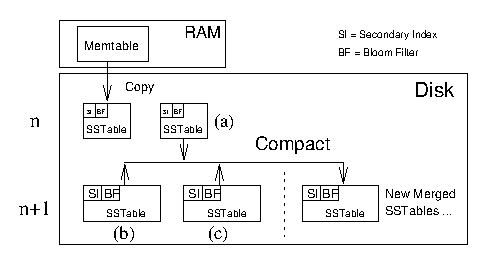
\epsfig{file=figures/leveldb-compact.eps,width=1.00\linewidth}
\caption{LevelDB Compaction}
\label{fig:compact}
\end{centering}
\end{figure}

To serve a key lookup, Memtable is queried firstly. If not found in
Memtable, the SSTables are queried in reverse chronological order. A
naive implementation of such a lookup can be very slow because the
whole database need be read and checked in the worst case. To make
lookup fast, SSTable are organized into several layers with the size
of each table increasing from the top layer to the bottom. Background
jobs are launched periodically to sort and merge small SSTables into
larger ones in the next layer. This is called compaction. Deleted
pairs are also removed during compaction. Then a lookup iterates the
SSTables layer by layer and returns once the key is found.  Because
SSTables are sorted by key, it enables fast lookup algorithm like
binary search. There is also index for SSTables tells the key range
covered by a particular SSTable so that it suffice just checking the
SSTables whose key ranges cover the interested key. Inside each
SSTable, we can have a bloomfilter to filter negative key lookup and a
secondary index for faster search.

In LevelDB, there are two Memtables, once one is filled, the other one
is used for further insertion. The filled one is flushed into a
Memtable in background. Its compaction procedure is illustrated in
Figure~\ref{fig:compact}. One SSTable (a) at layer $n$ is merged with
the SSTables at layer $n+1$ that have overlapping keys with (a) into
new SSTables at layer $n+1$.

\subsection{Multi-Resolution Image}
Multi-Resolution Images are different representations of the same
image at different resolutions. A common form of multi-resolution
images are images with different pixel resolutions, for instance,
thumbnails at $100\times100$, small images at $600\times800$, and
large images at $2048\times3072$. Multi-Resolution also describes a
category of techniques used in image processing and
analysis~\cite{mrisimg}, including image pyramids (e.g., Laplacian
pyramids), discrete wavelet transform, and wavelet image compression.
Images are represented and stored with multi-resolution version not
only because for fast preview but also for extracting different level
of information from image content.

As we can see from Figure~\ref{fig:mrisidea}, we see a match of the
multi-resolution image and the storage tiers. The idea of MRIS is to
matching the storage system for the objects stored in it. It also
exploits the strength of different types of storage media.

\begin{figure}[t]
  \centering
  \begin{minipage}[l]{0.48\linewidth}
    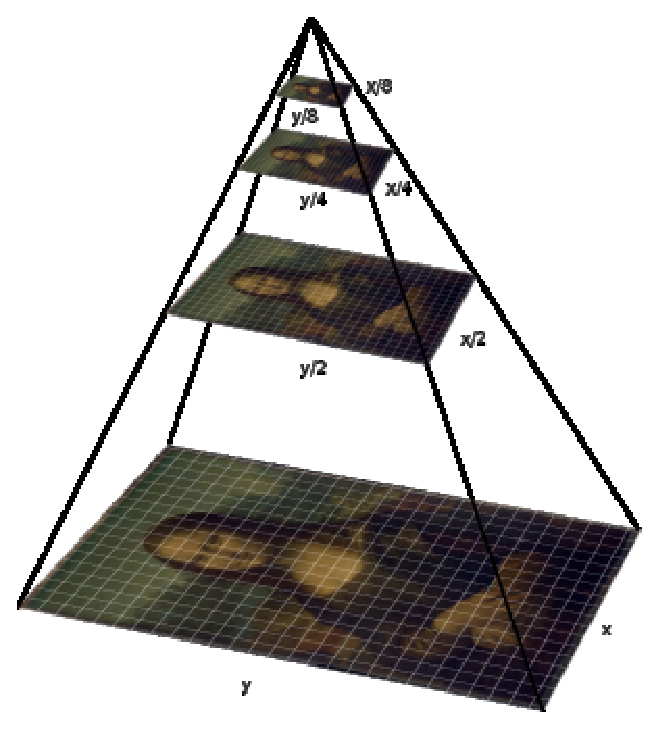
\epsfig{file=figures/pyramid.eps,width=.75\linewidth}
    \centerline{\footnotesize(a) Multi-Resolution Image}\medskip
  \end{minipage}
  \begin{minipage}[r]{0.48\linewidth}
    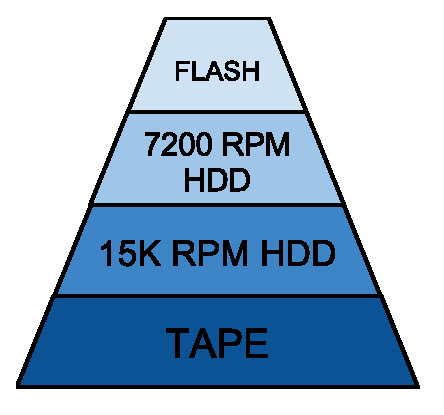
\epsfig{file=figures/storage-tiers.eps,width=0.9\linewidth}
    \centerline{\footnotesize(b) Storage Tiers}\medskip
  \end{minipage}
  \caption{Multi-Resolution Image and Storage Tiers}
  \label{fig:mrisidea}
\end{figure}

%Background...

%Typical length: 0 pages to 1.0.

%Background and Related Work can be similar.
%Most citations will be in this section.

%1. Describe past work and criticize it, fairly.  Use citations
   %to JUSTIFY your criticism!  Problem: hard to compare to YOUR
   %work, b/c you've not yet described your work in enough
   %detail.  Solution: move this text to Related Work at end of
   %paper.

%2. Describe in some detail, background material necessary to
   %understand the rest of the paper.  Doesn't happen often,
   %esp. if you've covered it in Intro.

%Example, submit a paper to a storage conference: reviewers are
%experts in storage.  Don't need to tell them about basic disk
%operation.  But if your paper, say, is an improvement over an
%already-advanced data structure (eg., COLA), then it'd make
%sense to describe basic COLA algorithms in some detail.

%Important: open the bg section with some "intro" text to tell
%reader what to expect (so experienced readers can skip it).

%If your bg material is too short, can fold it into opening of
%'design' section.


%\textbf{notes about picking a project}

%Put every possible related citation you can! (esp. if conf.
%doesn't count citations towards page size).

%Literature survey:
%- CiteSeer

%- Google Scholar

%- libraries

%1. find a few relates paper

%2. skim papers to find relevance

%3. search for add'l related papers in Biblio.

%4. reverse citation: use srch engines, to find
   %newer papers that cite the paper you like.

%5. "stop" when reach transitive closure

%- then go off and read it.

%- think about "how can I improve" and "what was so
  %good about that paper".

%- check future work for project ideas.

%- go to talks \& conferences

%Pick an idea:

%- novelty vs. incremental (how big of an increment?)

%- idea vs. practical implications
  %(implemented? released? in use as OSS or commercial?)

%- where to submit? good fit and match for quality.

%- look at schedule of conferences: due dates \& result dates.

%%%%%%%%%%%%%%%%%%%%%%%%%%%%%%%%%%%%%%%%%%%%%%%%%%%%%%%%%%%%%%%%%%%%%%%%%%%%%%
%% For Emacs:
% Local variables:
% fill-column: 70
% End:
%%%%%%%%%%%%%%%%%%%%%%%%%%%%%%%%%%%%%%%%%%%%%%%%%%%%%%%%%%%%%%%%%%%%%%%%%%%%%%
%% For Vim:
% vim:textwidth=70
%%%%%%%%%%%%%%%%%%%%%%%%%%%%%%%%%%%%%%%%%%%%%%%%%%%%%%%%%%%%%%%%%%%%%%%%%%%%%%
% LocalWords:  SMR HDDs drive's SMRs

\section{Design}
\label{sec:design}

\begin{figure}[ht]
\begin{centering}
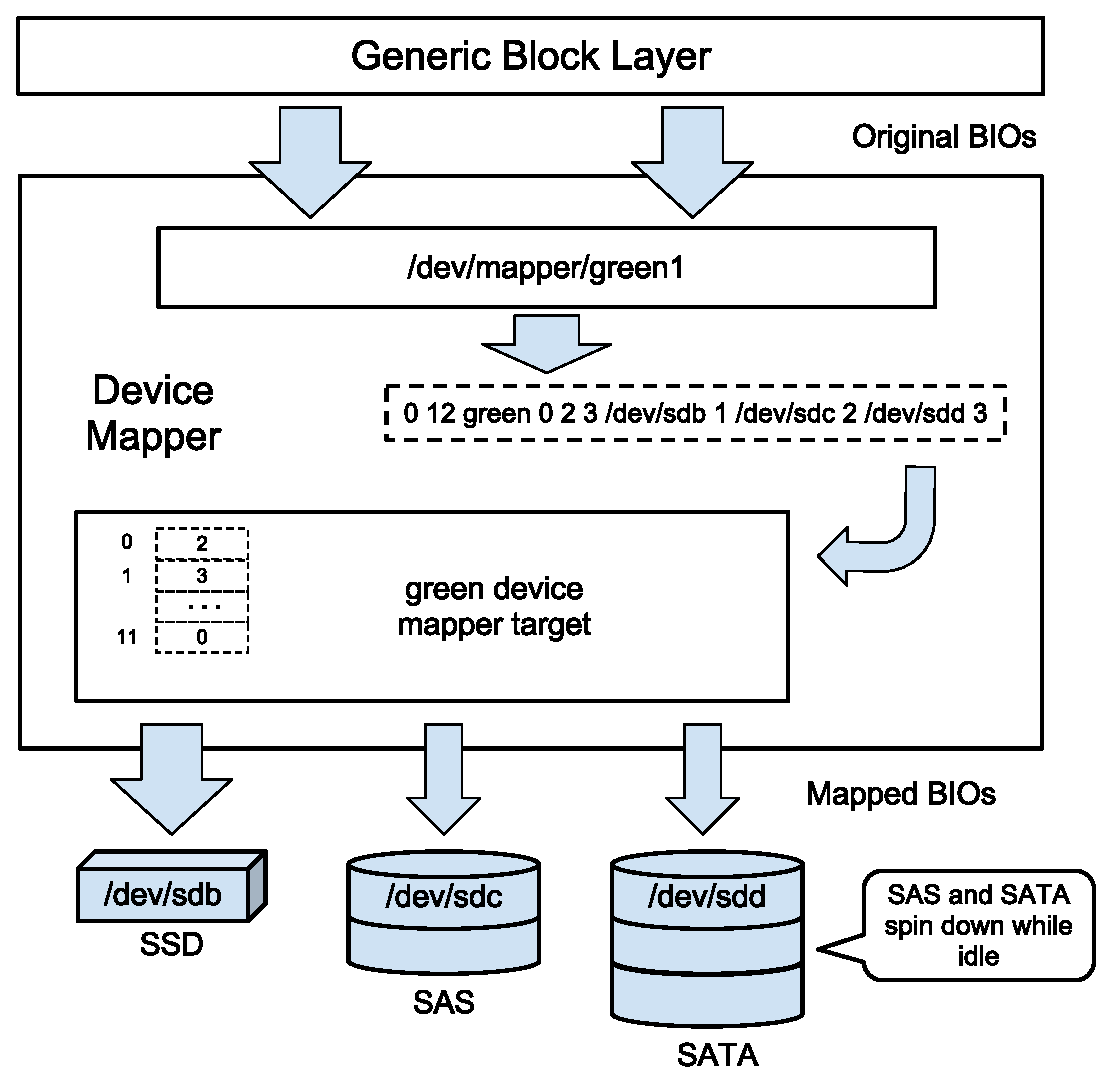
\epsfig{file=figures/dm.eps,width=1.00\linewidth}
\caption{Linux Device Mapper and Green Device Mapper Target.
\texttt{/dev/mapper/green1} is a virtual block device created by the
framework. The two dashed boxes are mapping tables. The first one is
used by the Device Mapper to delegate mapping to target; the second
one is used internally by the green target.}
\label{fig:dm}
\end{centering}
\end{figure}

We implemented our green multi-disk driver as a Linux Device Mapper
target. Linux Device Mapper, as depicted in Figure \ref{fig:dm}, is a
generic framework to map one block device onto another. It works by
processing data passed in from a virtual block device, that it itself
provides, and then passing the resultant data on to another block
device \cite{wiki_dm}. The advantage of Device Mapper is that it can
provide virtual devices to user programs and kernel modules above
block level without exposing underlying devices.  Thanks to this
transparency, the underlying devices can be of different size and type
(can in turn be virtual or physical) and the mapping can be performed
in a different manner. The Device mapper is essentially a middleware
sitting between the Generic Block Layer and block devices. It receives
BIOs, which are kernel structures describing I/O requests, from
Generic Block Layer, then redirect them to other block devices by
modifying the target device and sector offset. 

\begin{figure}[t]
\begin{minipage}[t]{.98\linewidth}
{\footnotesize
  \begin{tabular}{|p{0.9cm}|p{1.0cm}|p{0.9cm}|p{4.5 cm}|}
   \hline
   Offset & Length & Target & Target Parameters \\
   \hline
    0 & 524288 & linear & /dev/sdd 0  \\
    524288 & 1572864 & linear & /dev/sdc 0    \\
   \hline
  \end{tabular}
}
\centerline{(a) A mapping table using the linear target}
\end{minipage}
\begin{minipage}[b]{.98\linewidth}
{\footnotesize
  \begin{tabular}{|p{0.9cm}|p{1.0cm}|p{0.9cm}|p{4.5 cm}|}
   \hline
   Offset & Length & Target & Target Parameters \\
   \hline
   0 & 2097152  & green & 2 8 2 /dev/sdd 65536 /dev/sdc 196608 \\
   \hline
  \end{tabular}
}
\centerline{(b) A mapping table using the green target}
\end{minipage}
\caption{Two mapping tables used in our experiments. One table
corresponds to one virtual device. One entry of the table corresponds
to one range of the virtual device. Offset and Length are in unit of
sectors. Target Parameters are parsed by corresponding target.} 
\label{fig:dmtable}
\end{figure}

The Device Mapper itself does not perform the redirection. It
delegates this operation to Device Mapper targets, which are
registered kernel modules performing certain kinds of mapping. This
delegation is specified in a mapping table, which contains the types
of responsible Device Mapper target for different regions of the
virtual devices created by the framework. Figure \ref{fig:dmtable}
presents two examples. The first table is $524288+1572864$ sectors
large and contains two regions $[0, 524288)$ and $[524288,
524288+1572864)$.  Both of the two regions are handled by the linear
target. The first region maps all I/Os to \texttt{/dev/sdd} starting
from offset 0; the second region maps all I/Os to \texttt{/dev/sdc}
starting from offset 0 as well. The second table corresponds to a
virtual device that is 2097152 sectors large but contains only one
region. The region is handled by the green target.  Device Mapper
targets contain functions to construct/destruct virtual device
regions, map I/O requests, merge adjacent I/O requests, report and
control device status. Parameters of our green target start from three
integers (\texttt{2 8 2} in Figure \ref{fig:dmtable}(b)). The first
one is metadata mode. It tells how to initialize metadata when a
virtual device is created. There are currently three mode. Mode 0
means to create virtual device using metadata previously created on
disk and report failure if no metadata exists; Mode 1 means to use
existing metadata on disk but initialize new metadata if not exists;
Mode 2 means create brand new device and new metadata.  The second
parameter is the size of an extent in unit of sector, which is 8
sectors in the example. The third is the number of underlying physical
disks. The rest are pairs of physical device name and length of the
device in unit of extent. 

\subsection{Design Goals}
The design goal of our green multi-disk Device Mapper target is driven
by the following three guiding principles: 

\begin{enumerate}

\item \textbf{Save energy by allowing disks to spin/power down}.
Energy efficiency is one of the most important features our green
multi-disk target is pursuing. The SSD benefits both I/O performance
and energy efficiency simultaneously. In this study, we are more
concerned about the latter. We have made trade-offs between energy
efficiency and other desirable features such as capacity.

\item \textbf{Use SSD aware data structures and algorithms}. While SSD
provides better I/O performance and energy efficiency, it has its own
constraints including limited erase-write cycles and inefficient
random writes. This principle guides our design to avoid these
constraints and extract the maximum benefit out of an SSD.

\item \textbf{Provide stable and robust storage}. Because our green
target provides customized block mapping and data grouping, it is
critical to always perform correct translation from virtual to
physical blocks. It should not lose mapping information in case of
power failures.

\end{enumerate}

\subsection{Disk Management}

Device Mapper targets maintain mapping of sectors between virtual and
physical disks. The straightforward method is to maintain a
sector-wise mapping table. However, it is prohibitive because its size
is too large to fit in memory. For example, the size of the
sector-wise mapping table of a 1TB disk (512-byte sectors) is as large
as 8GB with 4-byte table entries. Storing the mapping table on disk
(even on SSD) is not an option because it is too slow to incur extra
I/Os. A solution is to divide disks into larger units. Here, we adopt
the term \textit{extent}, which is the unit of disk managed by LVM,
typically 4MB. Then the mapping becomes extent-wise and its size
diminishes to 1MB in the above example. This extent-wise mapping and
migration is encouraged by modern disks, almost all of which support
\texttt{multcount} feature \cite{speed_up}. \texttt{multcount}, short
for multiple sector count, controls how many sectors are fetched from
the disk in a single I/O interrupt. As claimed in \texttt{hdparm}
manual \cite{hdparm}: 

\begin{quotation}
When the \texttt{multcount} feature is enabled, it typically reduces
operating system overhead for disk I/O by 30-50\%. On many systems, it
also provides increased data throughput of anywhere from 5\% to 50\%.
\end{quotation}

In our green target, multiple physical disks are mapped as a single
virtual disk. The physical disks are linearly organized in the order
of energy efficiency, i.e., the most energy-efficient one goes first
and so on. In Figure \ref{fig:dm}, \texttt{/dev/sdb} is the most
energy-efficient one but with smallest capacity, i.e., SSD;
\texttt{/dev/sdc} and \texttt{/dev/sdd} follow decreasingly in energy
efficiency and increasingly in capacity. This makes the addressing of
physical sectors easy. An extent index and an offset within extent
would suffice. We have noticed the case that one I/O request on logically
sequential blocks might be mapped to multiple I/O requests on
physically non-sequential blocks. Namely, the translation is performed
per extent instead of per request. However, extent is of big size, so
it is unlikely that the extent-by-extent translation becomes a
performance bottleneck. Furthermore, the Device Mapper framework
provides an interface to merge adjacent I/O requests, which also
alleviates this problem.

The size of an extent is an important factor because it affects not
only memory consumption but also the granularity of mapping and data
migration. A large size of extent has the following effects: 

\begin{itemize} 

\item \textbf{Smaller mapping table}. As already discussed, the
adoption of extent makes the mapping table becomes extent-wise and
small. 

\item \textbf{More aggressive pre-fetch}. An energy-efficient disk
such as SSD have similar effect as disk cache. When a large extent of
data is moved onto SSD, it can be considered as an aggressive
pre-fetch. 

\item \textbf{Coarse-grained data migration among disks and more
sequential I/O}. Because the major latency of magnetic disks is seek
time, a larger sequential migration does not significantly slow down
the I/O. Moreover, with a large size of migration unit, there are
fewer I/Os because adjacent sectors are processed in batch. This is
beneficial to the lifetime of SSD as well considering its limited
erase-write cycles.

\item \textbf{High overhead}. Since an extent can represent several
sectors, more sectors I/O can be wasted in case of wrong prediction
thus adding overhead to the overall system. 

\end{itemize}

Physical extents are managed using a bitmap. The extents on SSD are
treated specially. Besides being recorded in the bitmap, they are also
linked in two lists, one for free extents and the other for used ones.
This facilitates and speeds up manipulation of the extents on SSD,
which happens frequently.

Different workloads might favor different extent sizes depending on
file sizes, I/O frequency and read-write ratio. Therefore, we make the
extent size a configurable parameter to the green target so that
different trade-offs can be made via configuration. 

%-----------------------------------------------------------------------------

\subsection{Mapping Table}

There are two mapping tables in Figure \ref{fig:dm}. One is actually a
configuration file used by the Device Mapper framework; the other
contains extent-wise mapping information used internally by our green
target. We discuss the second one next.

The straightforward structure of the mapping table is an array of the
size of extent number on all physical disks. Table
\ref{tab:greemtable} shows the structure of the table. The mapping
table is maintained in memory and can be cached, so its lookup is
fast. Besides mapping information, the table also contains other
fields including flags, timestamp of the latest access, and number of
total accesses (possibly distinguished read from write). Flags are
used to record states of extents, which include, for example, 1)
whether the extent is accessed or not recently; 2) whether the extent
is under migration or not; and 3) whether the extent is updated or not
when it is under migration. Timestamp of the latest access and number
of total access are used to predict hot extents.

\begin{table}[t]
{\footnotesize
\centering
\begin{tabular}{r|c|c|c|c|}
\cline{2-5}
\cline{2-5}
  & Physical & & Usage & \\ 
  & Extent ID & Flags & Counter & Timestamp \\
 Virtual Extent Index & 64 bits & 16 bits & 32 bits & 16 bits\\ \cline{2-5} 
 0 & 23 & \dots & \dots & \dots \\
 1 & 9 & \dots & \dots & \dots \\ 
 \vdots & \vdots & \vdots & \vdots & \vdots \\ 
 511 & 234 & \dots & \dots & \dots \\ \cline{2-5}
  \end{tabular}
}
 \caption{Mapping table used by green target. The mapping of virtual
extent $i$ is recored at the $i$-th entry in the table.}
\label{tab:greemtable}

\end{table}

The mapping table needs to be saved onto disks on power off as
metadata. To be fail-safe, it has a replica in every physical disk.
The in-memory version and on-disk version of the mapping table can be
slightly different, since it is not necessary to save online
information such as the timestamp of latest access. To be robust in
case of power failures, the mapping table is flushed onto disk
periodically. To prevent this periodic background job from disturbing
secondary disks' idle periods, this flush saves the table only onto
the cache disk. Tables on other disks are only updated on request or
when the system is being shut down.

%-----------------------------------------------------------------------------

\subsection{Extent Migration}\label{sec:migrate}

The ideal case of our green target is that most I/Os are served using
only the SSD. We try to achieve this by keeping hot extents on the
SSD. However, hot extents are not fixed, they change over time. As an
cold extent becomes hot, we try to migrate it to the SSD. To
accommodate this migration, we have to move an extent on the SSD out if
the SSD was full. Essentially, one migration swaps two extents, one 
extent on one of the secondary disks which becomes hot, and one extent 
on the cache which becomes cold. In total, it involves two reads and 
two writes. To be consistent, incoming I/Os on the migrating extents 
are delayed until the migration is finished.  This elongates latency 
and hurts I/O performance. The following pseudocode describes the 
Read/Write path in using the green target.

To minimize the latency introduced by migration, we divide migration
into two separated operations, promotion and demotion. Promotion moves 
a hot extent from secondary disk onto the SSD, whereas demotion moves 
a cold extent on SSD to secondary disk. We perform demotion operation 
beforehand to ensure that SSD always has free extents available on it,
so that when an promotion operation comes, migration happens straight
away without the need for any other demotions.  In this way, we reduce 
the latency by performing this operation in advance.  Without the division
of demotion and promotion, we need 1) find a cold extent on the SSD,
2) move the cold extent out of the SSD, and 3) bring the hot extent
onto the SSD.  Demotion consists of operation 1 and 2; promotion
consists of operation 3.  

To put demotion ahead, we keep a set of the coldest extents on the
SSD, replicate them on the one of the secondary disks, and mark their
slots on the SSD as available.  When there is a promotion, we
consume one of the available slots and move the hot extent there.  By
consuming one of the available slots, we simply update the mapping of
the old extent to its replica on the secondary disk. In case one of
the extents we maintained as the coldest becomes hot before its slot
is consumed, we move it out of the set and invalidate its replica if
it has been written.

A background thread is used to perform demotion. It makes sure the
size of the set within a range, which is defined by a maximum
threshold and a minimum threshold. Demotion is scheduled when the size
falls under the minimum threshold. This ensures that available extents
can be readily obtained when promotions are needed. Once demotion
kicks start, it keeps demoting more extents until the maximum threshold
is reached. When the range is large, this strategy disturbs secondary
disks less frequently because it batches demoting. Therefore, the
secondary disks are kept idle for longer periods.  It costs space for
the replicas and requires reserved space to make sure there is always
free space. However, the cost is insignificant because they are on
cheap and large secondary disk. 

To find cold extent on SSD, we use the LRU heuristic. Because we can
find cold extents beforehand, we are allowed to use sophisticated LRU
algorithms to obtain good prediction. To predict hot extents, we adopt
a greedy approach and take the extents have just been accessed as hot.
A trade-off between I/O performance and SSD lifetime is possible when
promoting an extent being written. Because SSDs have limited
erase-write cycles, it makes sense to directly map writes to the
secondary disks instead of promoting the extent all at once. If that
extent is read immediately, then we promote it. This is helpful in
case of operations like file copying and file appending, where the
disk is written just once. This does not have a significant impact on
energy efficiency because the secondary disk hosting that extent has
to spin up no matter if we promote it right now or not.  Once it is
up, there is a relative long timeout before it can spin down again
because of the large penalty (latency and short disk lifetime) of disk
spin-down, so no additional spin-up is needed if that extent is read
soon.  Actually, there is research trying to extend SSD lifetime by
using HDD as write cache \cite{hddcache}.  However, this is a
configurable feature that allows users to make informed decisions when
workload knowledge is available. 

\subsection{Data Grouping}

We have studied the data grouping in Wildani et al's work
\cite{Wildani_grouping}, wherein data grouping is workload specific
and is performed offline. A simple heuristic we are going to
experiment is to group data by frequency of access. That is, most
accessed data are all mapped onto the first disk, namely, SSD and so
forth. The reason behind this is that it is likely for data in same
working set to exhibit access frequency at the same level.  Thanks to
our dynamic mapping, we can perform data grouping online as well. Our
migration favors data grouping.  It is likely that extents in a common
working set becomes cold at a same time. It is also likely that they
are demoted onto a single secondary disk instead of being scattered
among multiple disks because our demotions are processed in batch. 

%%%%%%%%%%%%%%%%%%%%%%%%%%%%%%%%%%%%%%%%%%%%%%%%%%%%%%%%%%%%%%%%%%%%%%%%%%%%%%
%% For Emacs:
% Local variables:
% fill-column: 70
% End:
%%%%%%%%%%%%%%%%%%%%%%%%%%%%%%%%%%%%%%%%%%%%%%%%%%%%%%%%%%%%%%%%%%%%%%%%%%%%%%
%% For Vim:
% vim:textwidth=70
%%%%%%%%%%%%%%%%%%%%%%%%%%%%%%%%%%%%%%%%%%%%%%%%%%%%%%%%%%%%%%%%%%%%%%%%%%%%%%
% LocalWords:  

\section{Implementation}
\label{sec:implementation}

\begin{figure}[t]
\begin{centering}
\epsfig{file=sstable.eps,width=1.00\linewidth}
\caption{SSTable}
\label{fig:sstable}
\end{centering}
\end{figure}


We implemented MRIS using LevelDB~\cite{leveldb-web}, an open source
key/value database engine developed by Google. LevelDB is
log-structured and organizes data into Sorted String Table (SSTable).
SSTable, introduced in Bigtable~\cite{chang06osdi}, is an immutable
data structure containing a sequence of key/value pairs sorted by the
key as shown in Figure~\ref{fig:sstable}. Besides key and value, there
might be optional fields such as CRC, compression type etc. SSTable
are mostly saved as files and each of them can contains data
structures, such as bloomfilter, to facilitate key lookup. SSTable
have counterpart in the memory called Memtable. The key/value pairs in
Memtable are often kept in data structures easy for insert and lookup
such as red/black tree and skiplist.

LevelDB, as well as most other key/value engines, use Log-Structured
Merge Trees (LSM)~\cite{lsm} for internal storage. When key/value
pairs are first added, they are inserted into Memtable.  Once the size
of the Memtable growes beyond a certain threshold, the whole Memtable
is flushed out into a SSTable, and a new Memtable is created for
insertion. When key/value pairs get changed, the new pairs are
inserted without modifying the old pairs. When key/value pairs get
deleted, a mark of the deletion is inserted. This way key/value can
provide large insertion throughput because data is written out using
sequential I/Os, which have good performance on Hard Disk Drives
(HDD). 

To serve a key lookup, Memtable is queried firstly. If not found in
Memtable, the SSTables are queried in reverse chronological order. A
naive implementation of such a lookup can be very slow because the
whole database need be read and checked in the worst case. To make
lookup fast, SSTable are organized into several layers with the size
of each table increasing from the top layer to the bottom. Background
jobs are launched periodically to sort and merge small SSTables into
larger ones in the next layer. This is called compaction. Deleted
pairs are also removed during compaction. Then a lookup iterates the
SSTables layer by layer and returns once the key is found.  Because
SSTables are sorted by key, it enables fast lookup algorithm like
binary search. There is also index for SSTables tells the key range
covered by a particular SSTable so that it suffice just checking the
SSTables whose key ranges cover the interested key. Inside each
SSTable, we can have a bloomfilter to filter negative key lookup and a
secondary index for faster search.

In LevelDB, there are two Memtables, once one is filled, the other one
is used for further insertion. The filled one is flushed into a
Memtable in background. Its compaction procedure is illustrated in
Figure~\ref{fig:compact}.

%%%%%%%%%%%%%%%%%%%%%%%%%%%%%%%%%%%%%%%%%%%%%%%%%%%%%%%%%%%%%%%%%%%%%%%%%%%%%%
%% For Emacs:
% Local variables:
% fill-column: 70
% End:
%%%%%%%%%%%%%%%%%%%%%%%%%%%%%%%%%%%%%%%%%%%%%%%%%%%%%%%%%%%%%%%%%%%%%%%%%%%%%%
%% For Vim:
% vim:textwidth=70 noai nocin nosi
%%%%%%%%%%%%%%%%%%%%%%%%%%%%%%%%%%%%%%%%%%%%%%%%%%%%%%%%%%%%%%%%%%%%%%%%%%%%%%
% LocalWords:  SSTable LevelDB Memtables

\section{Trace Study}
\label{sec:trace}

Traces are used to collect information about the system workloads.
Traces can be collected at different layers in the storage stack.
Block traces contain information about disk offset, number of blocks
accessed, read/write information, and timestamp for every accessed
I/O.  This information can be used to characterize the workloads and
identify I/O access patterns.  Trace analysis plays a crucial role in
identifying hot data blocks across different disks. The idea is to
move hot blocks to the cache disk and use it to serve most of the
requests. Hence other disks can be spun/powered down for long periods
of time to achieve good power savings and increased performance. A
simple approach like counting the number of times a particular block
is accessed can be used to find the hotness of disk blocks. Apart from
this, I/O block traces can be used for a variety of other purposes.
For example, block-trace analysis can be used to tweak the design
parameters like extent size and migration threshold.

Workloads that exhibit good data locality properties are most suitable
for this project. Workloads such as video server and file server are
likely to exhibit this property. The distribution of popular files on
disks may change dynamically but at any particular instant, only a
fraction of files are popular in the case of above workloads. A
workload which is completely random I/O access patterns could not
benefit this approach as it could result in frequent data migration
between primary disks and secondary disks.
 
Currently, we use I/O traces for analysis and tweaking parameters. I/O
traces can also be used in offline mode to predict the hot blocks.
This approach is another option and we may implement this if time
permits. Also, to verify the correctness and working of our concept,
we replay the traces with and without green Multi-disk target and
compare the power consumption and I/O performance. 

\begin{figure}[ht]
\begin{centering}
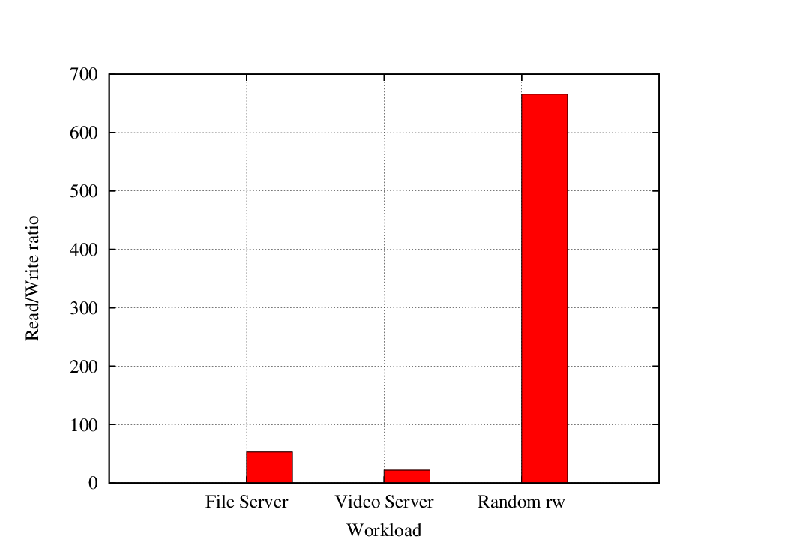
\epsfig{file=figures/rw.eps,width=1.00\linewidth}
\caption{Read/write ratio of video server, file server and random
  workloads.}
\label{fig:rwratio}
\end{centering}
\end{figure}

\begin{figure}[ht]
\begin{centering}
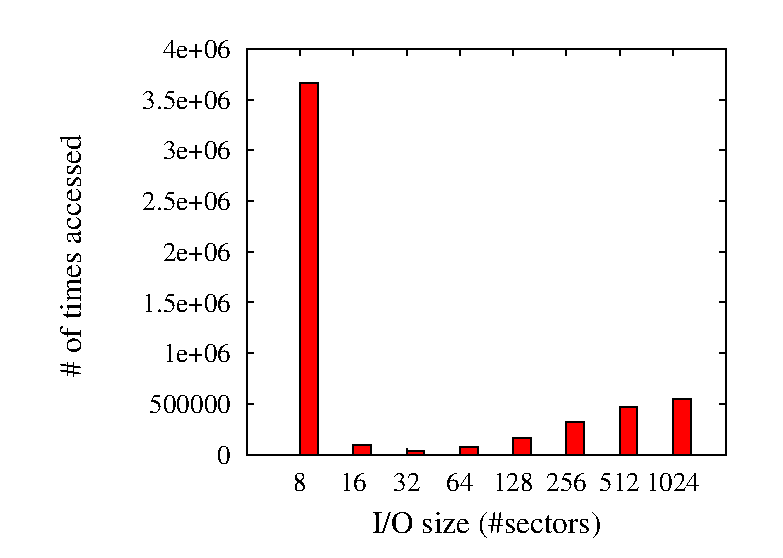
\epsfig{file=figures/trace_iosize.eps,width=1.00\linewidth}
\caption{I/O size and number of access of the videoserver workload.
Generated by Filebench when the I/O size parameter is set to be
random. Sizes are round to 512.}
\label{fig:randomiosize}
\end{centering}
\end{figure}

We have collected I/O block traces for workloads including video
server, file server, and random workloads. The workloads were run for
a relatively long periods (for a few hours). Below, we present the
results for some preliminary analysis on the traces. Figure
\ref{fig:rwratio} shows Read/Write ratios for the above three
workloads.  We have collected the number of times a particular I/O
size was issued for the above three workloads. Figure
\ref{fig:randomiosize}, which shows the I/O size of the video server
workload, is one of them. All these workloads were generated using
Filebench and each workload runs for 2 hours. We used three different
physical disks with different power consumption and performance
characteristics to run these workloads.  We noticed that a large
portion of the I/O sizes is 8 sectors. That is because most writes to
disk are schedules by \texttt{pdflush}, which write dirty pages (4K in
size) back onto disks periodically. 

%%%%%%%%%%%%%%%%%%%%%%%%%%%%%%%%%%%%%%%%%%%%%%%%%%%%%%%%%%%%%%%%%%%%%%%%%%%%%%
%% For Emacs:
% Local variables:
% fill-column: 70
% End:
%%%%%%%%%%%%%%%%%%%%%%%%%%%%%%%%%%%%%%%%%%%%%%%%%%%%%%%%%%%%%%%%%%%%%%%%%%%%%%
%% For Vim:
% vim:textwidth=70
%%%%%%%%%%%%%%%%%%%%%%%%%%%%%%%%%%%%%%%%%%%%%%%%%%%%%%%%%%%%%%%%%%%%%%%%%%%%%%
% LocalWords:  SMR HDDs drive's SMRs

\section{Evaluation} \label{sec:eval}

We have evaluated our system on a 64-bit Dell server with 1GB memory
and a one-core Intel(R) Xeon(TM) CPU 2.80GH CPU. The OS, a Ubuntu
server 8.04 with kernel version 3.2.9, is installed on a Maxtor
7L250S0 3.5-inch SATA HDD. We used the same but another SATA HDD and
one Flash based SSD for MRIS store. The HDD is also a Maxtor 7L250S0
with a capacity of 250GB and a rotational speed of 7200 rpm.  The SSD
is an Intel SSDSA2CW300G3 2.5-inch with 300G capacity.  The code and
benchmark results are publicly available at
https://github.com/brianchenming/mris.

\subsection{Measure drives}
\label{sec:drives}

Firstly, we measured the two storage devices used in our benchmarks.
The results we got support our argument that Flash is good in random
I/O while HDD is not bad in sequential I/Os. We formated both devices
using Ext4. We remount devices before each benchmark to make sure that
all disk caches are dropped. The devices were measured using
Filebench~\cite{filebench-web}. Random read and write were measured
using Filebench built-in workloads \texttt{randomread} and
\texttt{randomwrite}; Sequential read and write were measured using
Filebench built-in workloads \texttt{singalstreamread} and
\texttt{singalstreamwrite}.

\begin{figure}[t]
\begin{centering}
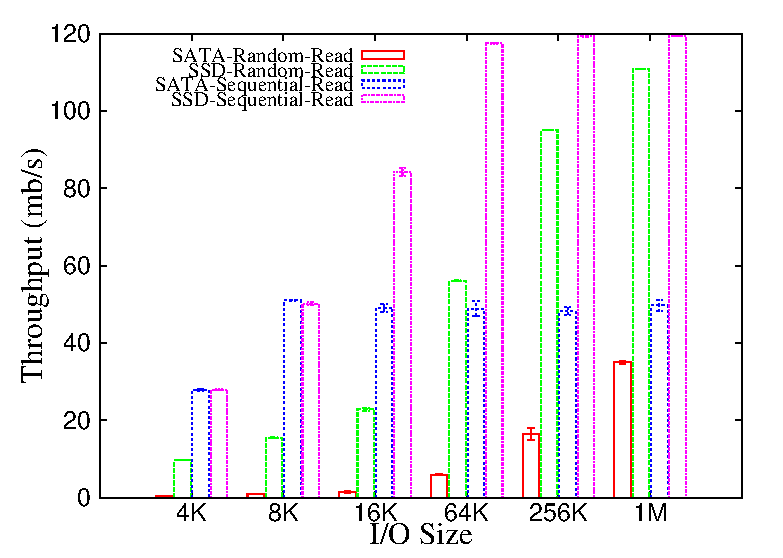
\epsfig{file=figures/ssd_vs_sata_read.eps,width=1.00\linewidth}
\caption{Read performance of SSD and HDD}
\label{fig:driveread}
\end{centering}
\end{figure}

The performance of read operations are presented in
Figure~\ref{fig:driveread}. All benchmarks are performed for 3 times,
and the standard deviation of the 3 runs are shown as error bar in the
figures. The results are stable and most error bars are imperceptible
or negligible. As we can see in Figure~\ref{fig:driveread}, SSD is
much better than that of HDD for random read for small I/O sizes. SSD
is 23.1$\times$ faster than HDD when I/O size is 4K, and 18.4$\times$
faster when I/O size is 8K. However, the speed advantage drops to
8.4$\times$ and 4.8$\times$ when the I/O size grows to 64K and 256K.
This is because disk head seek happens less frequently as I/O size
increases. Specifically, the HDD read throughput is 0.4mb/s with an
I/O size of 4K. This agrees with the 9ms average read time shown in
the HDD's specification.  

For sequential read, the most interesting observation is that HDD
provided the same throughput as SSD when I/O size is 4K and 8K. HDD
throughput stop grow after 8K, whereas SSD throughput grows until
256K. 8K and 256K are the points when HDD and SSD achieve their
respective maximum bandwidth.

\begin{figure}[t]
\begin{centering}
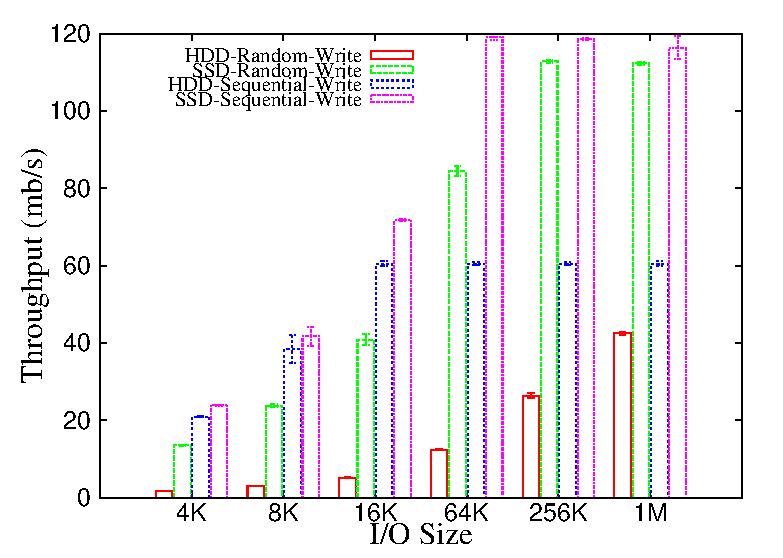
\epsfig{file=figures/ssd_vs_sata_write.eps,width=1.00\linewidth}
\caption{Write performance of SSD and HDD}
\label{fig:drivewrite}
\end{centering}
\end{figure}

The performances of write operations are presented in
Figure~\ref{fig:drivewrite}. They present similar trend as of read.
When I/O size is small (i.e. 4K, 8k, or 16k), SSD performs much better
than HDD for random write, but their performance have no significant
difference for sequential write. When I/O size becomes large,
throughput of both drives are capped by their maximum bandwidth.
However, we noticed that HDD performs better for write than for read.
This is because the HDD has a 16MB internal cache, which is more
helpful for write than for read. 

Above-mentioned results will serve as baselines of throughput for our
further benchmarking. They also validate our design premise that SSD
performs much better than HDD for random I/Os and HDD performs well
for sequential I/Os.

\subsection{Wikipedia Image Workload}

\begin{figure}[t]
\begin{centering}
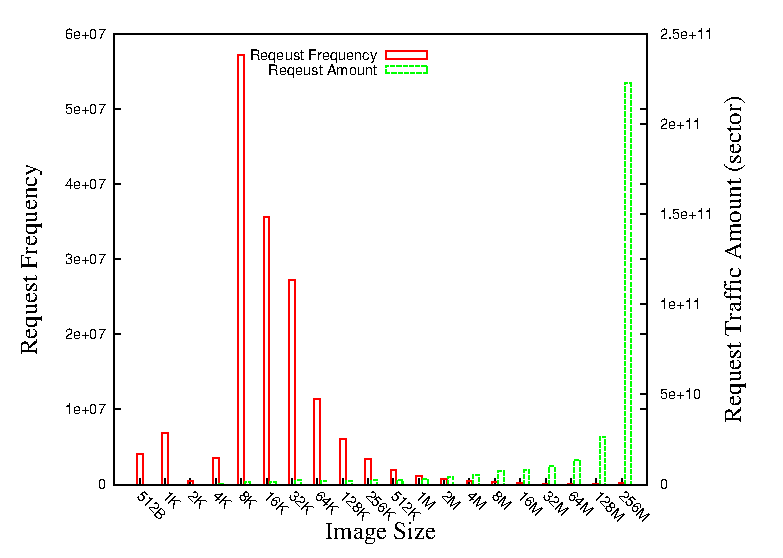
\epsfig{file=figures/wiki-image.eps,width=1.00\linewidth}
\caption{Image Requests to Wikipedia of January 2012}
\label{fig:wikiimage}
\end{centering}
\end{figure}

To study the size-tiered property in workloads, we analyzed the
requests of images made to Wikipedia site.  Wikipedia is the \#5
website in the world~\cite{wikipedia-web}, serving 492 million people
every month~\cite{wikimedia-foundation}. It can reflect workloads of
many large websites.

Figure~\ref{fig:wikiimage} presents the requests of images made in
January 2012. They are extraced from request log files from
http://dumps.wikimedia.org/other/pagecounts-raw/2012/2012-01/. We
extract requests of objects with a suffix of jpg, png, or gif, then
round up their sizes into power of 2. The frequency of images of
different sizes is counted and plotted in Figure~\ref{fig:wikiimage}.
All images larger than 256M is counted in the 256M bin. The first
observation from Figure~\ref{fig:wikiimage} is that the request image
of different sizes vary widely.  Particularly, images of sizes between
$(4, 64]$ KB are most popular. They sum to 81.58\% of the total number
of image requests. Moreover, 94.57\% of the requests are for images
smaller than or equal to 128KB. Despite the fact that small images
(smaller than 128KB) are the absolute majority in term of request
numbers, the traffic (size$\times$frequency) introduced by them is
just 2.96\% of the total. Although not all the requests make their way
to the storage layer because of memory cache (such as
Memcached~\cite{memcached}).  This salient size-tiered property of
requests still makes size-tiered storage a close match for
multi-resolution image workloads.

\subsection{MRIS Write}

%The drives were formatted using ext2, whereas fig:drivewrite was
%using ext4. This should not have happened. We need to redo one of the
%two sets of benchmarks in the future.

%TODO: specify that keys are not counted.

We now show micro benchmark results on simple workloads of sequential
and random write of multi-resolution images. Multi-resolution images
of the same content are often created from a common source. Therefore,
they are inserted into the image store at the same time. For example,
In Facebook's Haystack~\cite{beaver2010finding}, four resolutions,
thumbnail, small, medium, and large, are created from each image
uploaded by customers. As most images are in compressed format, we
emulate the workload of writing MRI by inserting groups of random
objects into MRIS with compression disabled. To be simple, each group
consists of two objects, both of which are random strings. One of the
two objects is 8KB large representing a small image, whereas the other
is 128KB large representing a large image. The SizeThreshold is set to
128KB, so that the large one will be stored in LargeSpace.

\begin{table}[tc]
{\centering \footnotesize
\begin{tabular}{c|c|c}
\hline 
  Setup & \multicolumn{2}{c}{Placement of Objects} \\ \cline{2-3}
   Name & Small (in SSTable) & Large (in LargeSpace) \\ \hline
  SSD & SSD & SSD \\
  Hybrid & SSD & HDD \\
  SATA & HDD & HDD \\ \hline 
\end{tabular}
 \caption{Setups For Benchmarking. The three setups differ in the
 places objects are stored.}
\label{tbl:setups}
}
\end{table}

Figure~\ref{fig:mriswrite} presents the results of the workload of
inserting 10,000 groups of objects into MRIS. We experimented the
workload on three different setups in Table~\ref{tbl:setups}. The
groups were inserted in random and sequential ways considering the
order of the key of objects. For ops/sec of random insertion, SSD is
28\% faster than SATA and Hybrid is 8\% faster than SATA. Considering
only SSD and SATA, the speedup of SSD is much lower than that shown in
Figure~\ref{fig:drivewrite}. This is because of the Memtable and the
log-structured feature of MRIS, which turns many random writes into
fewer large sequential write. It also explains how random writes
achieved a throughput of 23.9mb/sec even for SATA. As we can see in
Figure~\ref{fig:drivewrite}, SSD is only slightly faster than SATA
when it is for sequential write of 4K I/O size. Therefore, a slow
speedup of insertion is reasonable.

For sequential insertion, SSD is 26\% faster than SATA and Hybrid is
just 3\% faster than SATA. This is because sequential insertion causes
less compactions than random insertion, which reduce the overall
number of I/Os.  Compations merge multiple sorted SSTable into one
larger sorted SSTable. When key/value pairs are inserted sequentially,
no merge is necessary because all SSTable have no overlapping keys.
This also explains why sequential insertion is significantly faster
than random insertion for all the three setups (41\%, 38\%, and 45\%
faster for SSD, Hybrid, and SATA). 

\NOTE{Ming}{I really should have recorded the number of compactions
happened during the benchmarking. I will probably do it in several
days.}

% How fdatasync determines which I/O size to use? We will have to
% double check the I/O size. LevelDB has an internal block size
% defaults to 4KB, but that is not necessarily the I/O size.

% LevelDB writes SSTable using mmap and fdatasync. It is better if we
% can get some basic drive benchmarks using mmap in the future.

Figure~\ref{fig:mriswrite} (b) also shows throughput in term of
mb/sec.  However, the speed-up ratio of mb/sec is almost identical to
that of ops/sec (differ in less than 0.1\%). This is what we are
expecting because the average size of an operation is the same among
all setups.

\begin{figure}[t]
  \centering
  \begin{minipage}[c]{\linewidth}
    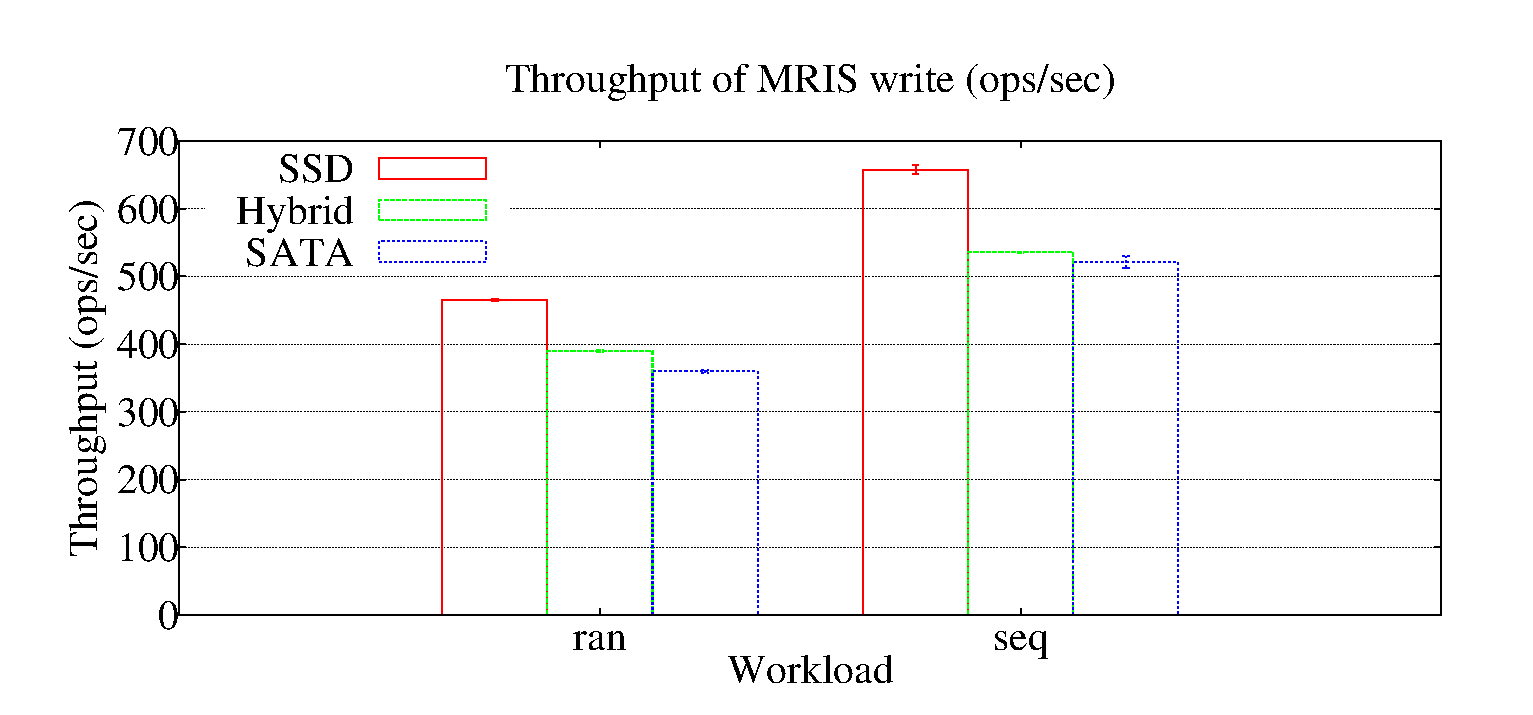
\epsfig{file=figures/mris-write-ops.eps,width=1.00\linewidth}
    \centerline{\footnotesize(a) Objects written per second}\medskip
  \end{minipage}
  \begin{minipage}[c]{\linewidth}
    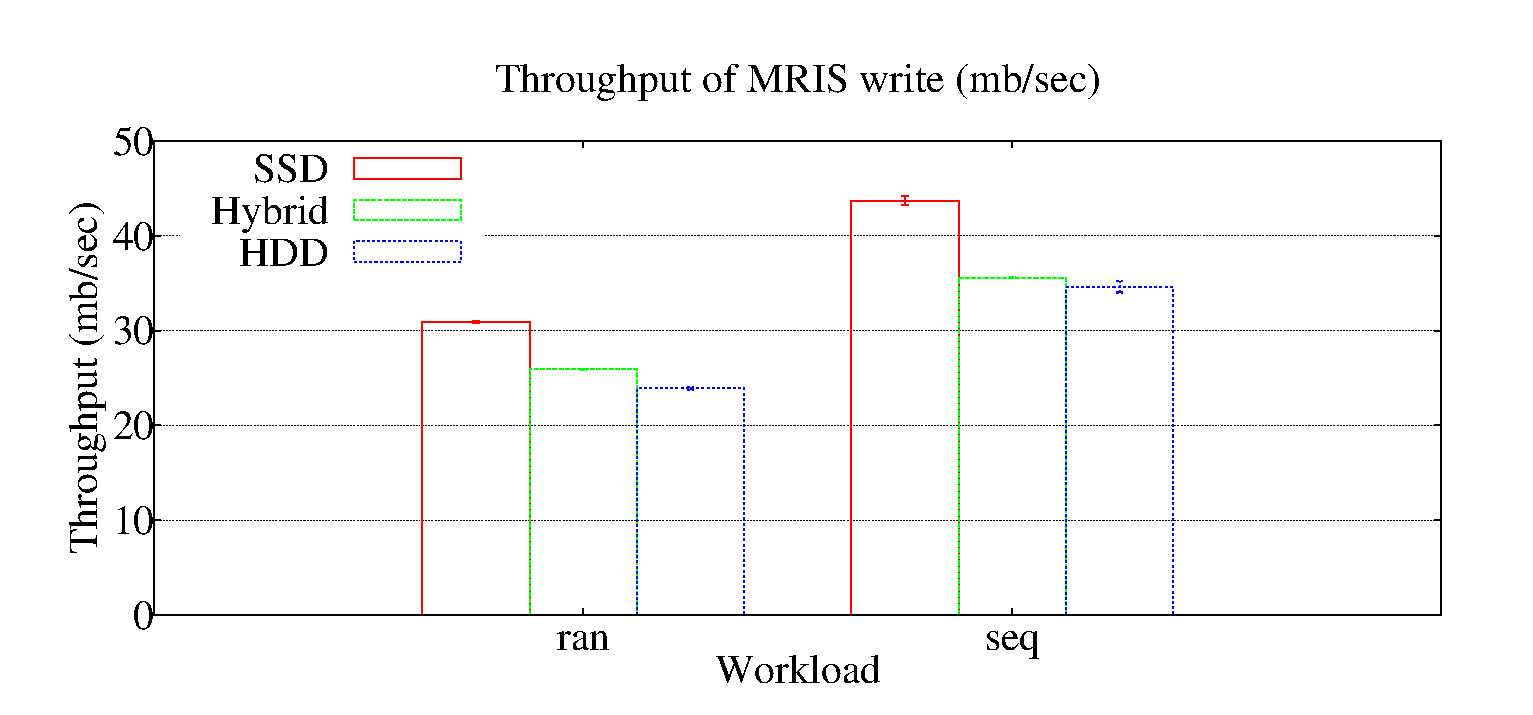
\epsfig{file=figures/mris-write-thput.eps,width=1.00\linewidth}
    \centerline{\footnotesize(b) MB written per second}\medskip
  \end{minipage}
  \caption{Write performance of MRIS.}
  \label{fig:mriswrite}
\end{figure}

\subsection{MRIS Read}

Log-structured key/value stores generally have high insertion
throughput, however, they also have to provide satisfactory lookup
performance.  We have developed workloads to evaluate the read
performance of MRIS.  One of the most intersting parameters in read
benchmarking is the ratio of reading small and large images. In
Facebook's workload~\cite{beaver2010finding}, the ratio of requests of
small and large images is around 17 (not considering thumbnails and
medium). In Wikipedia's workload, the ratio of requests of 8K-image
and 128K-image is around 9.5. In our benchmarks, we used different
ratios and performed workloads in all the three setups in
Table~\ref{tbl:setups}. Each benchmark randomly read 10,000 small
images from a database of 100,000 groups of images, and following
every $ratio$ reads of small images, one large version of the small
image is also read. For instance, one large image will be read after
every other read of small images when ratio is 2. This emulates the
common scenario that customers request large images once become
interested from the small ones.

\begin{figure}[t]
\begin{centering}
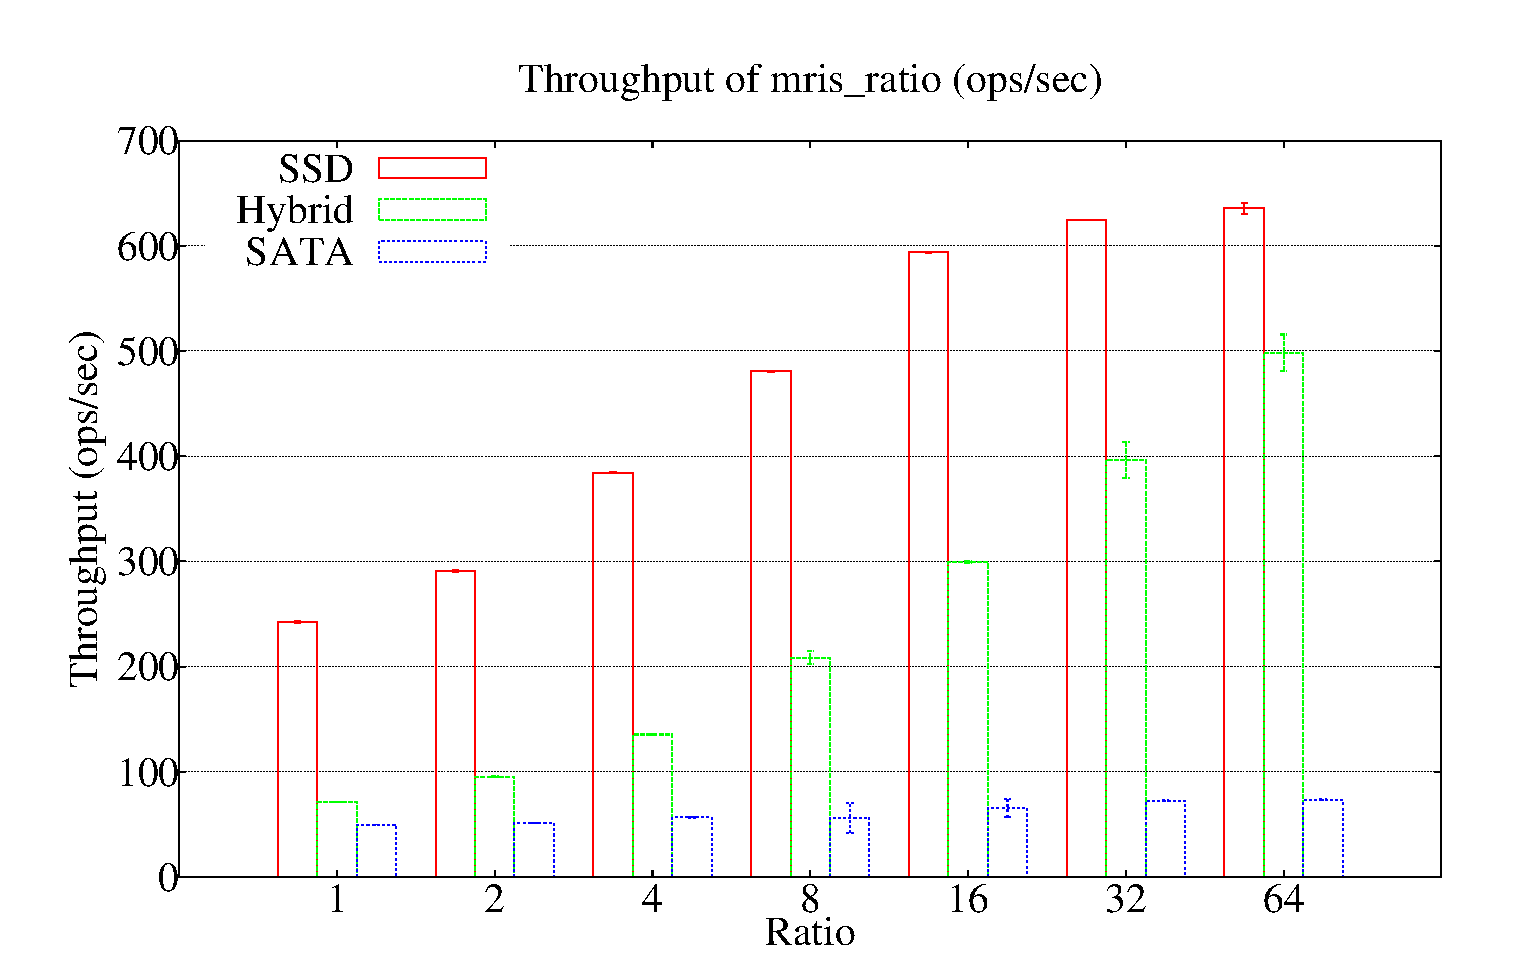
\epsfig{file=figures/mris_ratio_ops.eps,width=1.00\linewidth}
\caption{MRIS Read Performance (ops/sec). Each operation represents a
read of an image.}
\label{fig:mrisopssec}
\end{centering}
\end{figure}

Figure~\ref{fig:mrisopssec} presents the read throughput in term of
ops/sec. For all ratios, SSD shows the highest throughput among the
three setups, followed by Hybrid and then SATA. As shown in
Table~\ref{tbl:speedup}, the ops/sec of SSD is 3.89$\times$ to
7.64$\times$ faster than SATA. The speedup of SSD over SATA also grows
as ratio gets larger (except one point). This is because as the ratio
increases, the I/Os contain more small random reads, which exploits
more of SSD's superior random performance to SATA. Another interesting
observation is that the speedup of Hybrid over SATA grows rapidly from
0.44 to 5.78 as ratio increases.

\begin{table}[tc]
{\centering \footnotesize
\begin{tabular}{c|c|c|c|c|c|c|c}
\hline 
  Speedup & \multicolumn{7}{c}{Ratio} \\ \cline{2-8}
  over SATA & 1 & 2 & 4 & 8 & 16 & 32 & 64 \\ \hline
  SSD & 3.89 & 4.68 & 5.79 & 7.52 & 8.04 & 7.60 & 7.64  \\
  Hybrid & 0.44 & 0.86 & 1.39 & 2.69 & 3.56 & 4.46 & 5.78 \\ \hline
\end{tabular}
 \caption{Speedup of SSD and Hybrid over SATA (ops/sec).}
\label{tbl:speedup}
}
\end{table}

To help analyze the results, we use variables in
Table~\ref{tbl:variable} to represent the costs of involved read
operations in term of time. Then, ops/sec of SSD and SATA can be
expressed in (\ref{eqn:ssdops}) and (\ref{eqn:sataops}). 

\begin{equation}
\label{eqn:ssdops}
    1000000 \frac{ratio + 1}{t_{SF} * ratio + t_{LF}}
\end{equation}

\begin{equation}
\label{eqn:sataops}
    1000000 \frac{ratio + 1}{t_{SH} * ratio + t_{LH}}
\end{equation}

Using linear regression, we estimated the values of the variables
(also shown in Table~\ref{tbl:variable}) from our benchmark data.
Approxmiately, the ops/sec of Hybrid can be expressed in
(\ref{eqn:hybridops}).

\begin{equation}
\label{eqn:hybridops}
    1000000 \frac{ratio + 1}{t_{SF} * ratio + t_{LH}}
\end{equation}

\begin{table}[tc]
{\centering \footnotesize
\begin{tabular}{c|c|c}
\hline 
  Read Type & Flash SSD & SATA HDD \\ \hline
  Small Image & $t_{SF} = 1482$ & $t_{SH} = 13238$ \\ 
  Large Image & $t_{LF} = 6542$ & $t_{LH} = 37599$ \\ \hline
\end{tabular}
 \caption{Costs of read operations in time ($\mu$s). For instance,
$t_{SF}$ is the time of reading a Small image from the Flash SSD.}
\label{tbl:variable}
}
\end{table}

Use (\ref{eqn:hybridops}) and the values in Table~\ref{tbl:variable},
we can predict the ops/sec of Hybrid. The results, together with
measured ops/sec in our benchmarks, are presented in
Figure~\ref{fig:opspred}. We can see that the measured ops/sec
matches the shape of the predicted ops/sec. Moreover, the measured
ops/sec are all slightly higher than the predicted counterparts.

% TODO: measure the prediction accuracy with quantative metrics

\begin{figure}[t]
\begin{centering}
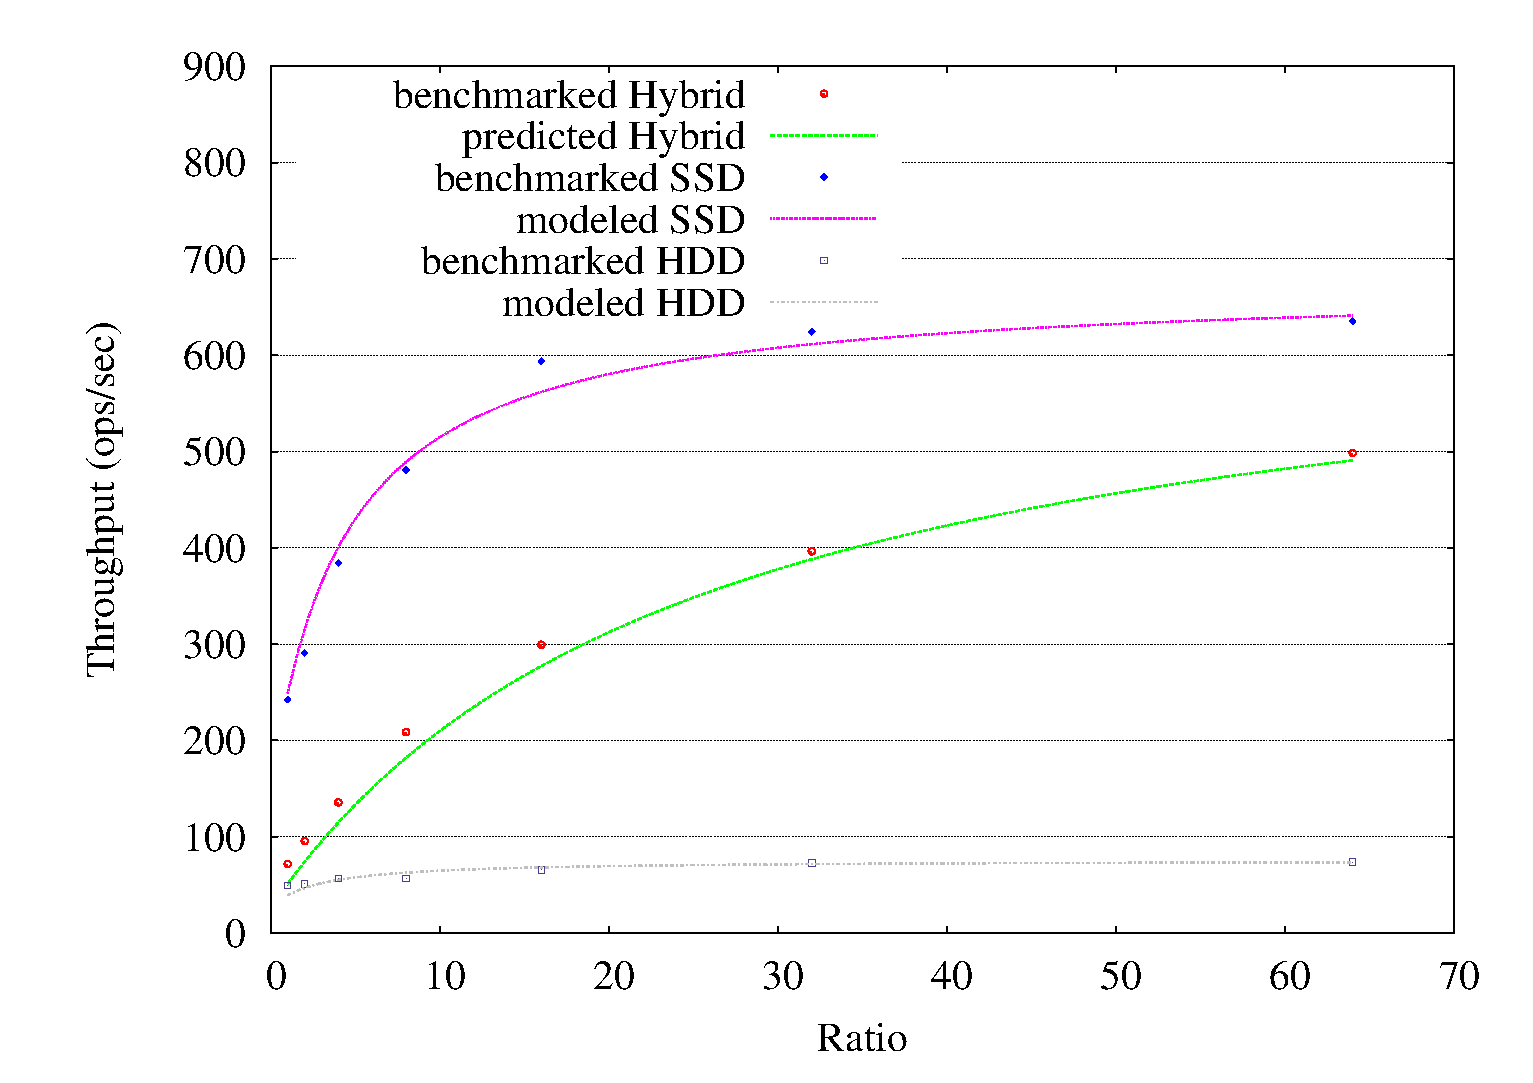
\epsfig{file=figures/ratio_ops_predict.eps,width=\linewidth}
\caption{Modeled and benchmarked performance (ops/sec).}
\label{fig:opspred}
\end{centering}
\end{figure}

For the same workloads, the throughputs in term of mb/sec are
presented in Figure~\ref{fig:mrismbsec}. Different from the results of
ops/sec, mb/sec is decreasing as ratio increases for both SSD and
SATA. This is because more of the operations are reads of small images
when ratio is large. As we can see in (\ref{eqn:opsize}), the average
size of an operation is a monotonically decreasing function of ratio
where $large = 128\mbox{KB}$ and $small = 8\mbox{KB}$ are the sizes of
large and small images respectively.

\begin{equation}
\label{eqn:opsize}
\begin{array}{r@{\quad=\quad}l}
  \mbox{avg\_op\_size} & \frac{ratio * small + large}{ratio + 1} \\
   & \mbox{small} + \frac{large - small}{ratio + 1} 
\end{array}
\end{equation}

\begin{figure}[t]
\begin{centering}
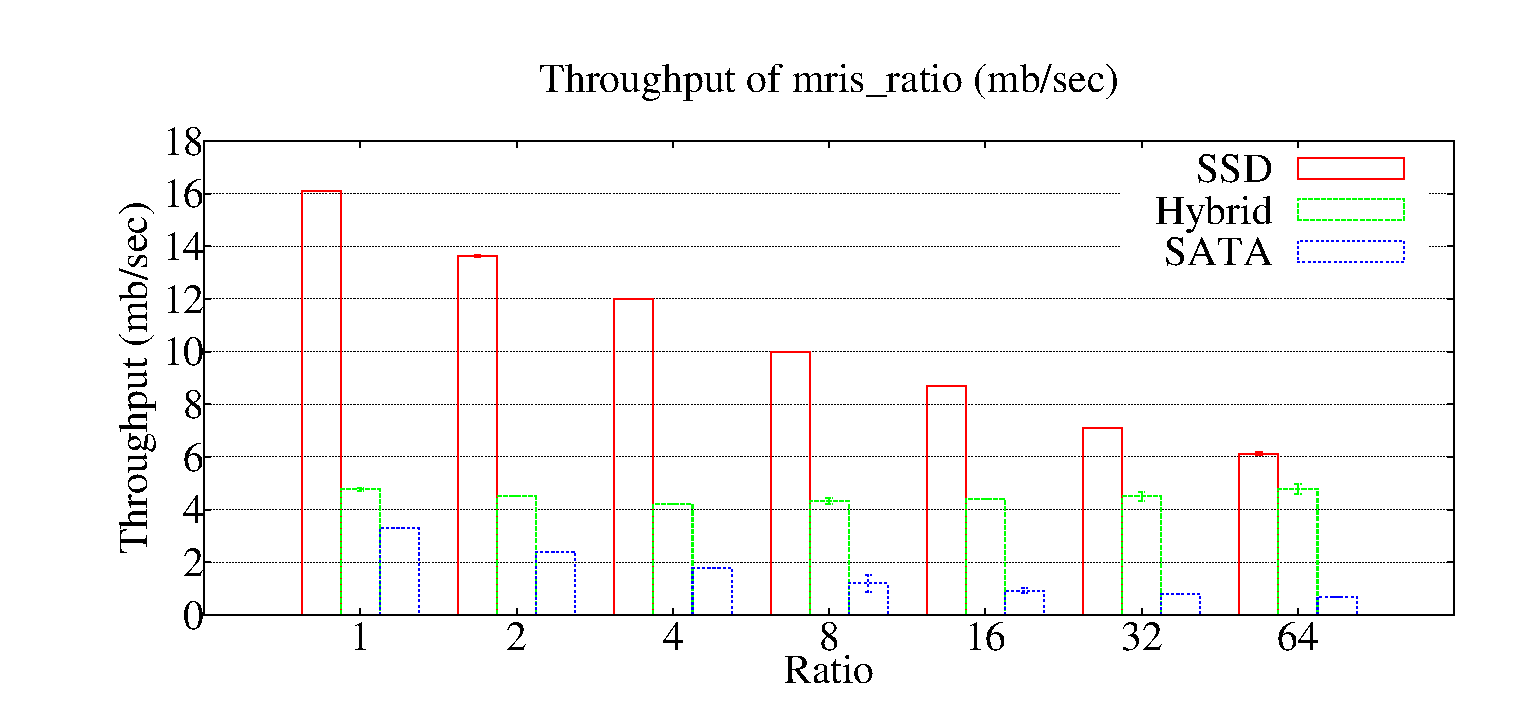
\epsfig{file=figures/mris_ratio_thput.eps,width=1.00\linewidth}
\caption{MRIS Read Performance (mb/sec).}
\label{fig:mrismbsec}
\end{centering}
\end{figure}

However, for Hybrid, the throughputs in Figure~\ref{fig:mrismbsec} are
relatively stable. Derived from (\ref{eqn:hybridops}), the mb/sec of
Hybrid can be expressed in

\begin{equation}
\label{eqn:hybridthput}
    1000000 \frac{ratio * small + large}{t_{SF} * ratio + t_{LH}} .
\end{equation}

Similarly, we can predict the mb/sec of SSD and SATA. The predicted
mb/sec results, along with the benchmarked mb/sec results, are
presented in Figure~\ref{fig:thputpred}. We observed that there exists
significant discrepancy in Hybrid's mb/sec results when ratio is
small. This is because the average operation size is large when ratio
is small, as we can see from (\ref{eqn:opsize}). The distances between
predicted ops/sec and benchmarked ops/sec of small ratios, in
Figure~\ref{fig:mrisopssec}, are magnfied when turned to mb/sec by
multiplying the average operation size.

\begin{figure}[t]
\begin{centering}
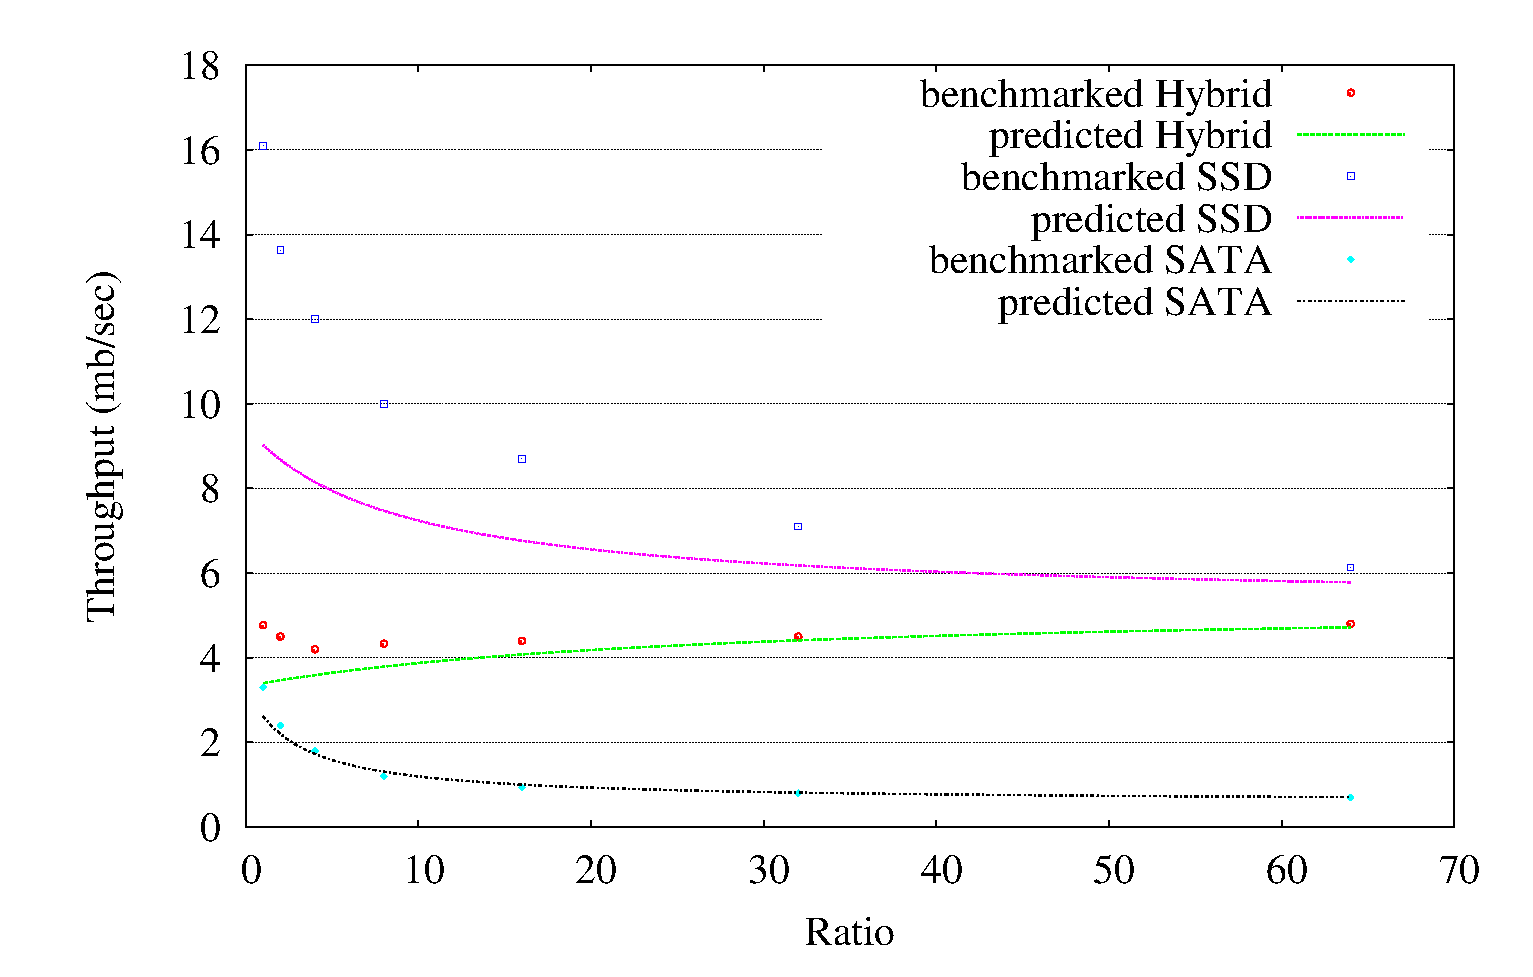
\epsfig{file=figures/ratio_thput_predict.eps,width=\linewidth}
\caption{Predicted and benchmarked read performance (mb/sec).}
\label{fig:thputpred}
\end{centering}
\end{figure}

As presented in Table~\ref{tbl:spdupmb}, Hybrid improves SATA's mb/sec
throughput by at least 45\%. The improvement grows to as high as
5.86$\times$ when ratio is 64.  Specifically, the speedup is
2.61$\times$ and 3.73$\times$ when ratio is 8 and 16, which
approximate to the ratios in the workloads of Wikipedia and Facebook.

\begin{table}[tc]
{\centering \footnotesize
\begin{tabular}{c|c|c|c|c|c|c|c}
\hline 
  Speedup & \multicolumn{7}{c}{Ratio} \\ \cline{2-8}
  over SATA & 1 & 2 & 4 & 8 & 16 & 32 & 64 \\ \hline
  SSD & 3.88 & 4.68 & 5.67 & 7.33 & 8.35 & 7.87 & 7.76 \\
  Hybrid & 0.45 & 0.88 & 1.33 & 2.61 & 3.73 & 4.62 & 5.86 \\ \hline
\end{tabular}
 \caption{Speedup of SSD and Hybrid over SATA (mb/sec).}
\label{tbl:spdupmb}
}
\end{table}

\NOTE{Ming}{TODO: consitify terms, such as images and objects, HDD and
SATA}

We have also measured the throughput (mb/sec) went to each drive using
iostat. The results are shown in Figure~\ref{fig:mrisiostat}. We
observed that the throughput reported by iostat is much larger than
that in Figure~\ref{fig:mrisopssec}. Three factors contribute to the
extra throughput: 1) the read-ahead in the filesystem, 2) extra read
of filesystem metadata, and 3) extra read of database metadata.
However, it is interesting to notice that the data read from SSD for
the SSD setup is quite stable even when ratio varies dramatically.
This is something we need to further investigate.

\begin{figure}[t]
\begin{centering}
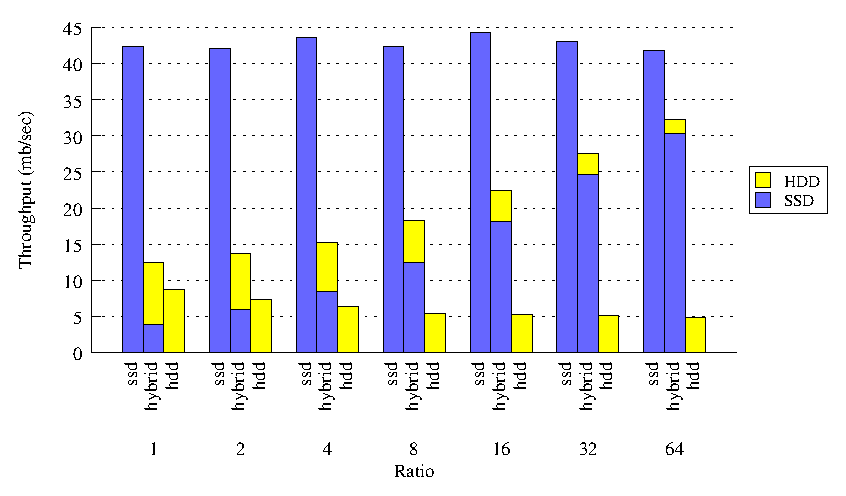
\epsfig{file=figures/mris_ratio_iostat_thput.eps,width=1.00\linewidth}
\caption{MRIS Read Performance (mb/sec) by iostat}
\label{fig:mrisiostat}
\end{centering}
\end{figure}

%%%%%%%%%%%%%%%%%%%%%%%%%%%%%%%%%%%%%%%%%%%%%%%%%%%%%%%%%%%%%%%%%%%%%%%%%%%%%%
%% For Emacs:
% Local variables:
% fill-column: 70
% End:
%%%%%%%%%%%%%%%%%%%%%%%%%%%%%%%%%%%%%%%%%%%%%%%%%%%%%%%%%%%%%%%%%%%%%%%%%%%%%%
%% For Vim:
% vim:textwidth=70 noai nocin nosi
%%%%%%%%%%%%%%%%%%%%%%%%%%%%%%%%%%%%%%%%%%%%%%%%%%%%%%%%%%%%%%%%%%%%%%%%%%%%%%
% LocalWords:  

\section{Related Work} 
\label{sec:related} 
Our work of optimizating performance of a key/value store using hybrid
storage devices is related to (1) hybrid filesystems, (2) multi-tier
storage, and (3) multi-level caching. 

\paragraph{(1) Hybrid Filesystems}

hFS~\cite{eurosys_hfs} is a hybrid filesystem which treats data
differently based on their size and type. Metadata and small files are
stored separately in a log partition like log-structured filesystem;
data blocks of large regular files are stored in a partition in a
FFS-like fashion. Similar to hFS, Conquest~\cite{conquest_tos} uses
battery-backed RAM to hold metadata and small files. Only large files
go to disk. Unlike hFS, UmbrellaFS~\cite{umbrellafs_gos} is a hybrid
stackable filesystem sit bellow VFS but above general filesystems such
as Ext2.  UmbrellaFS is able to use different devices including SSD.
TableFS \cite{tablefs} uses NoSQL store for metadata and small files.
However, its main objective is to improve the performance of a
filesystem using NoSQL store.

Whereas all of them integrate hybrid techniques into the filesystem
layer, our system lies in the application layer which is above the
filesystem layer. It optimizes the operations of an object store,
which provides a different interface from the POSIX filesystem
interface. This is an important difference because the filesystem
interface lacks application level knowledge, which is very useful in
optimizating application performance.

\paragraph{(2) Multi-tier Storage}
%
GTSSL~\cite{socc11chisl}

Flashup~\cite{vldb_flashup}

FAWN~\cite{sosp09fawn}

\paragraph{(3) Multi-level Caching}
%
Storage class memory such as Flash fills the gap between DRAM and HDD
in termns of cost, capacity and performance. It can be considered
either as backup for DRAM in the virtual memory layer or cache for HDD
in the block layer. Zhang et al.~\cite{zhang2012multi} and Saxena et
al.~\cite{flashvm} consider using Flash as backup of DRAM for paging,
whereas FlashTier~\cite{eurosys_12_flashtier},
FlashCache~\cite{flashcache} and Bcache~\cite{bcache} use Flash as
block level cache. Our work resides in neither the virtual memory nor
the block layer. It is agnostic to all the above-mentioned techniques.

Forney et al. \cite{Forney2002fast} proposed storage aware caching for
heterogeneous storage systems. They made memory cache aware of the
different replacement costs and partitioned the cache for different
storage devices.  However, their study is set in a different context
which is a network-attached disk system.  They did not consider data
placement among different drives, which is an important strategy of
our study.

%\cite{fast_12_deindirection} also treats metadata and data differently, and
%store them in virtual blocks and physical blocks respectively.

%hFAD \cite{Seltzer09hfad} described an tag-based object store API that
%supports full text search and it focused more on user interface. As
%our work is also able to provide tagging and text searching of
%metadata, we are more focused on workload specific performance
%optimization. Moreover, the design of hFAD is above block level
%storage, whereas our work integrate hybrid block level stroage
%techniques into our storage system.

%\cite{kvworkload_sigmetrics} strong locality metrics, such as keys
%accessed many millions of times a day, do not always suffice for a
%high hit rate; and there is still room for efficiency and hit rate
%improvements in Memcached’s implementation.  We found that the salient
%size characteristics follow power-law distributions, similar to
%other storage and Web-serving systems

%Why not cache in block level? Because block layer lacks the knowledge of
%objects and files.

%It may even be worthwhile to investigate not caching large objects at
%all, to increase overall hit rates \cite{kvworkload_sigmetrics}.

%%%%%%%%%%%%%%%%%%%%%%%%%%%%%%%%%%%%%%%%%%%%%%%%%%%%%%%%%%%%%%%%%%%%%%%%%%%%%%
%% For Emacs:
% Local variables:
% fill-column: 70
% End:
%%%%%%%%%%%%%%%%%%%%%%%%%%%%%%%%%%%%%%%%%%%%%%%%%%%%%%%%%%%%%%%%%%%%%%%%%%%%%%
%% For Vim:
% vim:textwidth=70
%%%%%%%%%%%%%%%%%%%%%%%%%%%%%%%%%%%%%%%%%%%%%%%%%%%%%%%%%%%%%%%%%%%%%%%%%%%%%%
% LocalWords:  SMR HDDs drive's SMRs

\section{Conclusions}
\label{sec:conc}
We present a multi-tier key/value store using Flash SSD and HDD. It
exploits the size-tiered feature in many workloads, especially the
multi-resolution image workload. It achieves good balance of
performance and cost by leveraging SSD's high random I/O throughput as
well as HDD's good sequential I/O performance. With a small Flash of
5.9\% of the total storage capacity, it is able to improve the ops/sec
of an emulated Facebook image workload by 3.73$\times$.

\paragraph{Future Work}
We plan to further study the model of multi-tier key/value considering
cost, characteristics of different drives, as well as more workload
specific features besides the ratio of read small and large objects.
More threads will be used in benchmark to exploit better parallelism
in Flash SSD.

\paragraph{Acknowledgement}
The author would like to thank Mike Ferdman, Vasily Tarasov, and Erez
Zadok for their valuable comments.

%%%%%%%%%%%%%%%%%%%%%%%%%%%%%%%%%%%%%%%%%%%%%%%%%%%%%%%%%%%%%%%%%%%%%%%%%%%%%%
%% For Emacs:
% Local variables:
% fill-column: 70
% End:
%%%%%%%%%%%%%%%%%%%%%%%%%%%%%%%%%%%%%%%%%%%%%%%%%%%%%%%%%%%%%%%%%%%%%%%%%%%%%%
%% For Vim:
% vim:textwidth=70
%%%%%%%%%%%%%%%%%%%%%%%%%%%%%%%%%%%%%%%%%%%%%%%%%%%%%%%%%%%%%%%%%%%%%%%%%%%%%%
% LocalWords:  

%\paragraph{Acknowledgments}
\label{ack}

1 pgf max.

Optional if you have space.  Cannot ack in anonymous
submissions.

List anyone who helped ideas, review drafts, but isn't a
co-author.

List any funding agency that supported the work (some agencies
require this).

Example:

We thank the EMC/Data Domain performance team for their help.  We also
thank Windsor Hsu, our shepherd Jiri Schindler and our anonymous
reviewers for their helpful feedback.  This work was supported in part
by NSF award CCF-0937854.



%%%%%%%%%%%%%%%%%%%%%%%%%%%%%%%%%%%%%%%%%%%%%%%%%%%%%%%%%%%%%%%%%%%%%%%%%%%%%%
%% For Emacs:
% Local variables:
% fill-column: 70
% End:
%%%%%%%%%%%%%%%%%%%%%%%%%%%%%%%%%%%%%%%%%%%%%%%%%%%%%%%%%%%%%%%%%%%%%%%%%%%%%%
%% For Vim:
% vim:textwidth=70
%%%%%%%%%%%%%%%%%%%%%%%%%%%%%%%%%%%%%%%%%%%%%%%%%%%%%%%%%%%%%%%%%%%%%%%%%%%%%%
% LocalWords:  SMR HDDs drive's SMRs

%\clearpage

% \appendix
% \input{appendix}

\bibliographystyle{plain}
\bibliography{template/master,gos}
%{\footnotesize \bibliography{template/master}}

%\newpage

\end{document}

%%%%%%%%%%%%%%%%%%%%%%%%%%%%%%%%%%%%%%%%%%%%%%%%%%%%%%%%%%%%%%%%%%%%%%%%%%%%%%
%% For Emacs:
% Local variables:
% fill-column: 70
% End:
%%%%%%%%%%%%%%%%%%%%%%%%%%%%%%%%%%%%%%%%%%%%%%%%%%%%%%%%%%%%%%%%%%%%%%%%%%%%%%
%% For vim:
% vim:textwidth=70
%%%%%%%%%%%%%%%%%%%%%%%%%%%%%%%%%%%%%%%%%%%%%%%%%%%%%%%%%%%%%%%%%%%%%%%%%%%%%%
% LocalWords:

% LocalWords:  Ankur Agrawal Benixon Arul Dhas Hospodor Yangwook Kang Rekha UC
% LocalWords:  Pitchumani Sphurti Sortur USletter csrg smr
